% Document template suitable for use as a LaTeX master-file 
% for thesis works in University of Turku Department of Computing
%
% Technical usage guide: https://tech.utugit.fi/soft/thesis/doc/doc/overview/
% 

\documentclass[language=english,version=draft,mainfont=none,sharelatex=false]{utuftthesis}
\setcounter{secnumdepth}{3}
\setcounter{tocdepth}{3}
\usepackage{float}
\usepackage[caption=false]{subfig}
\usepackage{graphicx}
\usepackage{multirow}
\usepackage{array}
\usepackage{hyperref}
\usepackage{longtable}
\usepackage[toc]{glossaries}
\graphicspath{ {./images/} }

% Define the algorithm environment
%\makeatletter
\providecommand\textquotedblplain{%
  \bgroup\addfontfeatures{Mapping=}\char34\egroup}
\providecommand{\tabularnewline}{\\}
\floatstyle{ruled}
\newfloat{algorithm}{tbp}{loa}
\providecommand{\algorithmname}{Algoritmi}
\floatname{algorithm}{\protect\algorithmname}
%\makeatother

\addbibresource{Bibliografia.bib}

\makeglossaries

\newglossaryentry{greensoftware}
{
    name=Green and sustainable software,
    text=green and sustainable software,
    description={Software that has a minimal negative or positive environmental, social, economic, and technical impact. This is achieved by continuously monitoring these aspects and optimizing them during development\cite{modelforselected}\cite{sustainabledevelopmentsustainablesoftware}}
}
\newglossaryentry{technicalsustainability}
{
    name=Technical sustainability,
    text=technical sustainability,
    description={The ability of software to adapt to future change~\cite{Calero2015}}
}
\newglossaryentry{economicalsustainability}
{
    name=Economic sustainability,
    text=economic sustainability,
    description={The ability of software development to shield stakeholders from economic risks~\cite{Calero2015}}
}
\newglossaryentry{environmentalsustainability}
{
    name=Environmental sustainability,
    text=environmental sustainability,
    description={The ability of software and its development to minimize the impact on the environment~\cite{Calero2015}}
}
\newglossaryentry{socialsustainability}
{
    name=Social sustainability,
    text=social sustainability,
    description={The ability of software to affect society positively and minimize negative effects~\cite{Calero2015}}
}
\newglossaryentry{individualsustainability}
{
    name=Individual sustainability,
    text=individual sustainability,
    description={The ability of software development to keep developers satisfied with their jobs~\cite{Calero2015}}
}
\newglossaryentry{issb}
{
    name=International Sustainability Standards Board (ISSB),
    description={Responsible for creating sustainability-related financial reporting standards}
}
\newglossaryentry{ifrs}
{
    name=International Financial Reporting Standards (IFRS),
    description={Offers standardized ways of producing financial statements for companies}
}
\newglossaryentry{rapl}
{
    name=RAPL,
    description={Running Average Power Limit. An interface for the CPU to report its energy consumption. Can be read by different monitoring programs}
}
\newglossaryentry{msr}
{
    name=MSR,
    description={Model Specific Register. A register in a CPU that exposes specific information about the CPU, for example, energy consumption}
}
\newglossaryentry{greeninit}
{
    name=Green in IT,
    text=green in IT,
    description={Sustainability improvements in IT regardless of the use case of the IT system in question. For example optimized code}
}
\newglossaryentry{greenbyit}
{
    name=Green by IT,
    text=green by IT,
    description={Sustainability improvements by IT systems. Systems whose functionality allows sustainability gains. For example energy management systems in buildings}
}
\newglossaryentry{pgo}
{
    name=PGO,
    description={Profile Guided Optimization. Allows compiler to better optimize software based on data collected from usage environments}
}
\newglossaryentry{embeddedemissions}
{
    name=Embedded emissions,
    text=embedded emissions,
    description={Emissions produced during the manufacturing and transportation of a product}
}
\newglossaryentry{sustainabilitydebt}
{
    name=Sustainability debt,
    text=sustainability debt,
    description={Debt that is accumulated in software projects that negatively affects its sustainability aspects~\cite{sustainabilitydebt}}
}
\newglossaryentry{csrd}
{
    name={Corporate Sustainability Reporting Directive (CSRD)},
    description={Mandates large corporations to report their emissions, including those from ICT systems~\cite{europaDirective20222464}}
}

\begin{document}

\pubyear{2024}
\pubmonth{0}
\pubtype{di}
\title{Adapting Sustainable Software Development Methods Into Agile Processes}
\author{Tuomas Rinne}

\maketitle
\keywords{green code, green software, sustainable software, agile, scrum}
\begin{abstract}
There is growing interest in developing software that is more sustainable technically and economically but also environmentally. The sustainability of software has been researched for over a decade and many methods for creating more sustainable software have been discovered. However, most development processes employing these methods have stayed on a theoretical level and practical implementations are hard to find. There are also many open questions about measuring the sustainability of software. This thesis presents a practical implementation of a sustainable software development process that also allows for measuring relevant sustainability metrics. A literature review was used to identify methods for creating sustainable software, existing agile methodologies for sustainable software, and relevant metrics and tools for measuring the sustainability of software. These findings were then added to a development model that splits the software development process into pre-development, development, usage, and post-development phases to facilitate sustainability in different phases of a software development project and measure relevant metrics in these phases. This model was then validated with existing literature on criteria for sustainable software development processes and with expert interviews. The result of this thesis is a development model that should produce more sustainable software and allow for the measurement of different aspects of sustainability with relevant metrics.
\end{abstract}

% mandatory
\tableofcontents

% if you want a list of figures
\listoffigures

% if you want a list of tables
\listoftables

% if you want a list of acronyms
\listofacronyms

\printglossary

% change the name if the default doesn't sound right
\renewcommand{\algorithmname}{\listingscaption}

% The thesis starts here.

% TOC Plan

\chapter{Introduction} \label{Introduction}
ICT systems are estimated to use about 7\% of all energy produced globally and this is estimated to grow to 13\% by 2030~\cite{europaPressCorner}. Additionally, energy prices are becoming more volatile~\cite{ieaGlobalEnergy}. There are also many geopolitical tensions connected to semiconductor manufacturing and rare metals needed for modern computers. EU has also passed the \gls{csrd} and the \gls{issb} has also mandated that every company following the \gls{ifrs} must report emissions including those from ICT systems~\cite{ifrsIFRSISSB}. All of this has led to more interest in \gls{greensoftware} which in part aims to maximize the potential of hardware to run software faster, cheaper, and with less computing power and energy required and also have tools to measure the energy consumption of software accurately.

The idea of \gls{greensoftware} development has been around for a long time. Some parts of \gls{technicalsustainability} such as technical debt and \gls{economicalsustainability} such as the cost of developing and running software are well-known factors in the software development industry. Recently the \gls{environmentalsustainability} has also seen more interest. There are studies from 2011~\cite{greensoft} presenting ideas on creating software more sustainably and as far back as 2001 for estimating the impact of ICT on the environment~\cite{ictimpact}. Despite this, the energy usage of ICT is growing and remains a concern~\cite{theimpactofinformationtechnology}. \Gls{greensoftware} often requires making code more efficient by optimizing it. Unfortunately, this has historically been seen as more difficult and expensive than just buying more hardware when scaling the software to more users. The problem of rising system requirements without apparent benefit for the software being used has been known for a long time and is often referred to as Wirth's Law~\cite{wirth}, which states that any advantages gained from faster hardware are negated by software becoming slower.

\section{Challenges in Sustainable Software}\label{challenges}
There are many open challenges in developing sustainable software. Lack of standard interfaces, metrics, configurations, and tools are often mentioned~\cite{Challenges}~\cite{empiricalstudyonpracticioners}~\cite{miningquestions}. There is also a general lack of awareness and knowledge on the topic of sustainable software among developers~\cite{softwareindustryawarness} and how to measure energy consumption~\cite{energyefficiencyanewconcern}. There is also relatively little research on sustainable software and how to apply it in practice as most of the existing research is very theoretical~\cite{Nurmivaara2023}. This can make it hard to create guidelines for developing sustainable software. This thesis aims to address some of these challenges by providing some guidelines, metrics, and implementations of different steps of existing development processes to facilitate more sustainable software development.

\section{Goal}
The goal of this thesis is to create a sustainable agile development process primarily for use at Kvanttori, a small-sized software development company. This means that the model mainly focuses on web development and primarily aims at team sizes of 2 to 10 people.

\section{Research Questions}
This thesis aims to integrate sustainable software development practices into an existing agile software development process to produce more sustainable software by answering the following research questions:
\begin{itemize}
    \item RQ1: What methods are there for developing sustainable software?
    \item RQ2: How to measure the sustainability of the software?
    \item RQ3: How to integrate sustainable development methods into an agile development process?
\end{itemize}

\section{Research Methods}
A literature review is used to establish a clear understanding of the meaning of \gls{greensoftware} development and current agile development methods as well as documented methods for increasing and measuring the sustainability of software. A model for the agile development process is then created based on the findings of the literature review while also taking into account the current development model used at Kvanttori. The model should consider relevant methods for increasing software sustainability by reducing and measuring energy consumption and costs and by enhancing the technical aspects of software. In addition, expert interviews and existing criteria for sustainable agile processes are used to validate the usefulness of the proposed model.

The following query was used both on ACM and IEEE databases to find sources for the literature review: 

\begin{center}
\begin{tabular}{ |>{\centering\arraybackslash}m{\textwidth}| } 
\hline
\textbf{Query}\\
\hline
Green OR Sustainable  OR "Energy usage" OR "Energy efficiency" OR “Energy consumption” OR “Power usage” OR “Power consumption”\\
\hline
AND\\
\hline
Software OR Coding OR Code OR Programming OR Pipeline OR CI/CD\\
\hline
 AND\\
\hline
Measuring OR Analyzing OR Estimating OR Predicting OR Ranking OR Agile OR Development OR Engineering\\
\hline
AND NOT\\
\hline
Android OR IOS OR Mobile OR Phone OR Embedded OR IoT OR Cryptocurrency OR Building\\
\hline
\end{tabular}
\end{center}

This query excludes mobile, embedded, and IoT research as energy consumption has been a key issue in these domains for many years already due to battery constraints and they are not necessarily applicable to reducing energy consumption in domains where constant power sources are available. However, some energy-saving patterns can be ported from these devices~\cite{energypatternsforweb}. These patterns can be found by the snowball search method from found sources. Buildings and cryptocurrencies were excluded as their energy consumption is irrelevant to this thesis. This query, when limited to titles, yielded 113 results on ACM and 213 results on IEEE Xplore. From these, the most relevant were chosen by manual selection. The selected literature was also used as a starting point for the snowball search method to find the sources for information present in the research papers. ACM and IEEE were chosen since they have the most research papers relating to \gls{greensoftware} development~\cite{softwareengineerginaspectsofgreen}.

\section{Scope}\label{scope}
The development of \gls{greensoftware} is a broad subject that considers many parts of the development processes and organizations using them as well as different aspects of sustainability such as technical, economic, environmental, social, and individual sustainability. This thesis focuses on the sustainability of the software itself and as such will only briefly mention indirect effects of software development such as working environment, developer travel, and communications methods. The thesis aims to find what makes software itself sustainable, how to measure it, and how those aspects can be included in an agile development process. The complete sustainability impact of the software often also depends on the software's use case. A smart thermostat system that regulates temperature automatically can save a lot of energy regardless of how much energy running the software consumes. The focus of this thesis, as mentioned previously, is on \gls{greeninit}, not \gls{greenbyit}. This thesis mainly focuses on the technical, economic, and environmental aspects of sustainability as those can be the most affected within a single software project. While the social and individual sustainability aspects are affected in parts of the proposed model, measuring their impact is difficult within the context of a single project and is therefore left outside the scope of this thesis. Using the proposed development model in a project is also outside the scope of this thesis.

\section{Structure of the Thesis}
This thesis is split into 8 chapters. Chapter~\ref{Introduction} provides an introduction of the subject, research questions, and limitations in the scope of the thesis. Chapter~\ref{chapter2} defines \gls{greensoftware} in the context of this thesis and gives insight into what can be done to make software more sustainable. Chapter~\ref{chapter3} examines current agile software development methods and how they take efficiency into account as well as some existing research on incorporating sustainability into the agile development process. Chapter~\ref{chapter4} focuses on measuring the sustainability of software. Chapter~\ref{chapter5} introduces an agile framework for sustainable software development. Chapter~\ref{chapter6} contains expert interviews and results of trying to validate the framework with criteria found in the literature. Chapter~\ref{discussion} contains the answers to the research questions, threads to the validity of this thesis, and presents further research topics. Finally, Chapter~\ref{conclusion} contains the conclusion of the thesis.
\chapter{What Affects Software Sustainability?}\label{chapter2}
This chapter defines what is meant by sustainable software, what affects the sustainability of software, and why the sustainability of software is important. This chapter also answers \textbf{RQ1: What methods are there for developing sustainable software?} by listing methods for increasing the sustainability of software and its development.

\section{Criteria for Sustainable Software}\label{criteria}
One definition for \gls{greensoftware} is that it is software that has a minimally negative or even positive impact on the economy, society, and environment~\cite{modelforselected}. This takes into account the impact of all parts of the software lifecycle from the development process to the usage in a production environment to the eventual deprecation and replacement of the software. Another common definition for \gls{greensoftware} is software for which direct and indirect consumption of resources during different phases are monitored and optimized~\cite{sustainabledevelopmentsustainablesoftware}. For software to be sustainable, it should account for all different aspects of sustainability including \gls{technicalsustainability}, \gls{economicalsustainability}, \gls{environmentalsustainability}, \gls{socialsustainability} and \gls{individualsustainability}~\cite{Calero2015}.

Determining when exactly software can be called sustainable as many parts affect the sustainability of software and there is yet to be a single label or certification for \gls{greensoftware} that is commonly recognized. There are some efforts to create such labels. One of these labels is the Blue Angel label in Germany which applies to software products among many other types of products. So far only one software has this label~\cite{blauerengelBlueAngel}. There is also the MitViDi-criteria for public sector ICT projects that categorizes projects into one of three different classes depending on their sustainability requirements~\cite{mitvidi} and the Responsibility criteria for public procurement for software services~\cite{kriteeripankkiSoftwareServices} which is partly based on the MitViDi-criteria. These criteria can be used to introduce features and patterns promoting sustainability into software products even if these criteria are not yet commonly used.

\section{Methods for Developing Sustainable Software}\label{methods}
The sustainability of software, or how much the development and usage of the software affect the different sustainability aspects, is determined by both factors relating directly to the software, its development, and effects from its usage and also indirectly from the organization and its members who develop the software, their habits, and processes. Performance, efficiency, maintainability, portability, usability, and reliability have been identified as the most relevant characteristics for energy efficiency of software with performance being the leading indicator~\cite{systemicliteraturereview}.

Relevant energy efficiency characteristics also have an effect on the technical and economic aspects of sustainability as \gls{technicalsustainability} is directly affected by how maintainable the software is and \gls{economicalsustainability} is often affected by how much software costs to develop and run. Efficient software can run on less powerful and therefore less costly hardware. In services where usage is billed per hour, more performant software costs less to run. A core principle behind increasing the sustainability of software is to do less. This can manifest as doing less to achieve the same result, which is the case when using performant technologies and techniques such as caching, which allows using fewer CPU cycles to achieve the same result. It can also manifest as just doing less by not doing anything unnecessary. This can be achieved by requirements engineering and quickly dropping unnecessary features from the software.

Compared to performance, memory usage has little correlation~\cite{PEREIRA2021102609}\cite{10.1145/3136014.3136031}\cite{10.1145/3125374.3125382} with energy consumption. Lower memory usage might allow running more applications on the same hardware or running applications in more constrained environments, which in itself can make the software more sustainable so it should still be considered when optimizing for efficiency. Optimizing memory, not for lower memory consumption but rather for better usage of it for caching, can reduce the work the CPU needs to do and lead to faster execution, which in turn saves energy by preventing unnecessary work on the CPU. It should also be noted that optimizing for speed and memory are not redundant with each other so both should be targets for optimization~\cite{studyoninfluenceofsoftware}.

It should be noted that while performance has a strong correlation with energy efficiency, this is not always the case~\cite{towardsgreenranking}. For example, constantly running a CPU with maximum clock speeds is possible, theoretically resulting in the best performance but much worse energy consumption. However the correlation is strong enough that it can be used as a heuristic for efficiency~\cite{studyoninfluenceofsoftware}~\cite{energyefficiencyanewconcern}~\cite{twinsorfalseffriends}. As a general rule, the faster something runs, the less it does and by extension the less it consumes energy.

\subsection{Architecture}\label{architecture}
A well-thought-out architecture makes adding features more streamlined without the need to resort to workarounds that are sub-optimal from a performance standpoint. It also makes it easier for developers to follow good practices when implementing features. 

\subsubsection{Caching and Bulk Requests}
Software architecture can also be used to enhance performance by introducing cache systems and minimizing requests and database queries as these are always slower than querying in memory values. Generally, network and disk I/O traffic should be minimized. In addition, redoing work on the CPU should also be minimized.

Caches can help prevent unnecessary work by allowing the memoization of return values of functions so that the function does not need to run again if its arguments do not change. Caches can also be used to save values from network or I/O operations so that data does not need to be fetched again every time it is needed. ~\cite{guidelines}

Queries to resources over the network or on disk should be done in bulk when possible to get as much done in a single query as possible~\cite{guidelines}. This can make the application more performant and also lower costs in case used services for hosting are billed based on usage. Most databases have a way to do bulk requests or combine data from multiple tables with a single request.

\subsubsection{Data Structures and Algorithms}
Used data structures and algorithms can also have a great impact on energy consumption. Studies done with Java point to correct data structures having up to 11\% improvements in energy consumption~\cite{influenceofjava}. Another study showed that picking incorrect data structures can raise energy usage by over 300\% while optimizing can lower it by as much as 38\%~\cite{energyprofilesofjavacollections}. Algorithms and data structures should be optimized for speed rather than memory usage because the correlation between performance and energy consumption is much higher than the correlation between memory usage and energy consumption. Therefore data structures and algorithms with lower time complexity should be preferred.

\subsubsection{Error Handling}
 Error handling is also an important part of the architecture. Restarting a crashing application on errors will generally use more energy than handling errors gracefully. Error handling is also important for the maintainability of the software as handling errors in the same way and maybe even in the same place in code makes ensuring all errors are handled easier.
 
 \subsubsection{Logging}\label{logs}
 Not everything should be logged in running software. Unnecessary logs can cause performance slowdowns and unnecessary data transfer and storage. They can also make it more difficult to find relevant logs for specific issues.
 
 \subsubsection{Offloading}
 It can also be beneficial to offload heavy processing to a server in applications using a client-server architecture instead of running them on the client side~\cite{energyefficiencyanewconcern}. This can also help extend the lifespan of client devices as applications can have lower system requirements and do not require replacing client devices with more powerful ones to use the software.
 
 \subsubsection{Indexing}
 When planning the database architecture of the software, deciding what fields should be indexed for fast retrieval is important. This can significantly boost the performance of a database with the cost of some memory usage which should reduce the energy used by the database queries using indexed fields.

\subsection{Technology Choices}\label{technology}
Technology choices such as programming language, framework, and database systems can drastically affect energy consumption.

\subsubsection{Programming Language}
 Lower level and compiled languages tend to be much faster and more efficient, often in orders of magnitude, than interpreted languages~\cite{PEREIRA2021102609}\cite{10.1145/3136014.3136031}\cite{10.1145/3125374.3125382}. They also often result in smaller sizes for the software.

The choice of programming language affects more than just the performance. Languages with strong and static type systems can help prevent many issues that are typical to dynamically typed languages such as unexpected values. Some languages are also null safe, opting to use "Optional"-types instead, which can prevent unexpected crashes and other issues. Similarly, some languages handle errors as values instead of exceptions which makes it easier to ensure all error cases are handled. All of these attributes can greatly improve the \gls{technicalsustainability} of the software.

\subsubsection{Runtime}\label{runtime}
In interpreted languages the choice of the runtime can impact the performance for example when comparing the following production-ready JavaScript runtimes: Node, Deno, and Bun, there are great differences in their performance with Bun generally being the fastest and most energy efficient~\cite{snykNodejsDeno}~\cite{bunvsnodevsdeno}.

\subsubsection{Database}
 Some database systems such as relational databases like PostgreSQL can be drastically faster than document-oriented databases such as MongoDB~\cite{mongodbpostgresql}. Some databases also enforce much stricter typing of items put in them. Using these kinds of databases helps keep software maintainable by helping prevent mistakes caused by incorrect types.
 
\subsubsection{Libraries and Frameworks}
Even different libraries and frameworks can have drastic differences in speed despite using the same language~\cite{investigatingtheimpactofweb}. Newer and actively maintained frameworks tend to be faster as they leverage newer language features internally and have less technical debt which can be seen when comparing three Javascript web frameworks which are Express, Fastify, and Hono~\cite{webframeworksbenchmarkFrameworksBenchmark}. Express being much older is also slower than the other two.

\subsubsection{Large Language Models}\label{llm}
LLMs can use a lot of energy both when training and using them. Usage of these technologies should be carefully considered as they can also add a lot of complexity to the software. If these technologies are used, their impact should be mitigated. Using smaller, local models can reduce energy usage while also being faster and cheaper to run~\cite{greensoftwareGreenSoftware}.

\subsection{Size of Data}
The size of data directly affects the energy usage and performance when moving data via network or disk I/O. Therefore optimal datatypes should be used when moving files. Compression should also be used to minimize the size of data in transit and at rest~\cite{greensoftwareGreenSoftware}. Many backend services use JSON to move data but more efficient formats such as protocol buffers or CSV can be used to decrease the size of data~\cite{guidelines}. The used data format also depends on the complexity of the data as CSVs for example cannot be used to represent nested data.

File format is especially relevant in images as they are often large and can form a significant part of the data moved over the network in cases such as front-end applications. Newer formats such as WEBP and AVIF are much more space-efficient compared to formats such as JPEG and PNG and should therefore be used if possible. The image resolution is also an important factor. Images should be appropriately sized for their use case.

The size of the entire software is also an important factor when distributing it. Smaller software and updates use less energy when transferred over the network and are also faster to download. In some specific cases such as applications running on browsers, the size can be even more important than performance due to the software being fetched from the server every time it is used.

Data size should also be optimized when storing data. Using efficient formats and only storing what is needed can reduce the need for additional storage hardware~\cite{greensoftwareGreenSoftware}.

\subsection{Development Tools}
There are many tools that can be used during development to improve the sustainability of the software being developed. Automated testing and releasing can improve the quality of the software but they also affect the energy consumption of the development process.
Factors such as how often tools are run can cause unnecessary energy consumption during development. Furthermore, different testing and build systems can be drastically more efficient even within the same language ecosystem.

The energy consumed by development tools and tests can be affected by the efficiency of the software being built. Quality of implementation and chosen technologies will affect how long it takes for parts of the software and by extension tests to run. The required resources by testing environments also depend on the resource usage of the software. This will affect the cost of the testing environment and CI/CD pipelines.

Any tools used during the development are likely to increase the energy consumption of the development process. Software is often used much longer than it is developed. Therefore it makes sense to optimize the efficiency in the usage of the software even if the development consumes more energy as a result.

\subsubsection{Tests}
Tests can be used to maintain the technical quality of the software and catch issues early to prevent them from going into the production build of the software. Testing should be used to ensure that the software functions correctly.

Running unnecessary tests can decrease the sustainability of the development process by consuming more energy and costing more. Therefore only necessary tests should be run. The types of tests often depend on the project and therefore no general recommendation can be given on the types of tests.

\subsubsection{Benchmarks}
Benchmarks can be used to measure the performance of the software and should be used to ensure the software is fast and that there are no performance regressions in features.

At least the most used code paths should be benchmarked in addition to any performance-sensitive sections of the software.

\subsubsection{Formatters}
Formatters help keep the code consistent and easy to read. This helps improve maintainability as all code is at least mostly similar in every part of the software code.

Formatters should also be integrated into developers' editors to prevent developers from pushing unformatted code and causing CI/CD pipelines to re-run unnecessarily after failing on formatting issues.

\subsubsection{Linters}
Linters and other static analysis tools can catch issues during development resulting in a more sustainable final product but will likely increase the energy consumption of the development environment and CI/CD pipelines. Linters can also often be integrated directly into the code editors which can help catch issues early and prevent unnecessary CI/CD runs caused by these issues.

\subsubsection{Build Tools}
There are also other tools that can be integrated into the build process to enhance sustainability. Such tools include minifiers that allow optimizing the size of some static assets such as images. These tools allow automating image format conversions to more efficient formats which in turn reduces network traffic during the usage of the software.

\gls{pgo} is another build tool that allows collecting data from software and feeding it to the compiler during the build process to further optimize the software.

\subsection{Hosting}\label{hosting}
The devices running the software also have a significant impact on the sustainability of the software. In servers, the energy efficiency of the hardware used to run the software, virtualization, and things such as if the software is running all the time or started only when requests are made to it affect the energy usage and often the costs too. Virtualization allows fully utilizing hardware by splitting physical hardware into many virtual computers which allows maximizing the hardware use. There is also research in utilizing virtual machines to scale the number of servers that virtual machines run on depending on the load to optimize energy usage~\cite{virtualmachines}. 

Using serverless functions for some tasks can also save energy as they allow using hardware only when needed. However, research is conflicted on this as some research suggests serverless functions can increase the overall energy consumption by up to 15 times~\cite{serverless} while others suggest serverless platforms using up to 58\% less energy~\cite{serverless2}. These results indicate that the implementation of the serverless model is important and should be factored in when deciding to use serverless platforms.

When choosing a platform for hosting an application, the measurements provided by the hosting provider should be considered. Some services offer much more detailed metrics on resource and energy usage than others. Different hosting services also offer different services at different prices which affects the economical sustainability. They also have varying levels of support for different technologies in hosting platforms. 

The source of the energy used by hosting providers should also be considered. Green Web Foundation keeps a database of hosting providers that mainly use green energy to run their platforms~\cite{greenwebGreenFoundation}. It should also be noted that there are other factors such as the usage of heat from cooling and usage of water in hosting providers. This should also be considered if such information is available when making decisions about hosting services. 

Distance is also an important factor when discussing hosting providers. Applications should use servers that are as close to users as possible to minimize the distance data needs to travel as this also lowers the energy consumption and sometimes even the costs of running the software~\cite{greensoftwareGreenSoftware}.

Another important factor in hosting is the choice of hardware. Some providers allow running software on different CPUs, some of which might be more energy efficient~\cite{greensoftwareGreenSoftware}. The efficiency of the hardware is affected by how new it is and what architecture it uses.

\subsection{Configuration}\label{configuration}
Configuration used when building or bundling the software can also have drastic runtime performance impact~\cite{twinsorfalseffriends}. Optimization levels in some compilers for languages such as C and Rust can be used to optimize for speed or size and the difference between the lowest and highest optimization level can be great. In addition, optimizing for certain architecture levels to leverage instructions found in newer processors~\cite{phoronixBenchmarkingExperimental}. Therefore the target hardware should be taken into account when possible. Default configurations are often aimed at making the software work equally well on all supported platforms so it might make sense to change the configurations to optimize the build process to project specific target platforms.

Some web frameworks might use client-side rendering by default, or render pages every time on request if server-side rendering is enabled. These can often be configured to render specific pages that are not expected to change at build time and serve them to request preventing unnecessary rebuilding of pages on every request~\cite{greensoftwareGreenSoftware}.

\subsection{User Interfaces}
User interface and user experience design can also affect energy consumption. All functionality should require as few actions from the user as possible as this leads to less code being run and therefore saves energy and resources. This includes making the software accessible for accessibility tools. In addition, there should be easy ways to handle error situations and undo actions by the user. UI energy usage can also be reduced by using darker colors if client devices are expected to have OLED displays, which is often the case with smart TVs and smartphones, and by reducing the amount of animations and moving elements~\cite{energypatternsforweb}.

Optimizing for energy efficiency may require making trade-offs in user interfaces as animations and other decorative features can often increase energy consumption. These features might make the software stand out from the competition and can be important from a marketing perspective. The purpose of the software should be considered when designing the user interface. Simpler user interfaces should be preferred if it is not important to have one that stands out. In use cases where the user interface should stand out, elements with high energy consumption should be used sparingly to save energy while still being effective for their purpose. The effects of expensive visuals can also be mitigated by using smaller file formats and more efficient technologies.

\subsection{User Actions}
There is also some benefit in allowing users to disable features they do not need to save energy~\cite{energypatternsforweb}~\cite{mitvidi}. This could be for example allowing users to choose how many charts they want to see in an application showing different devices' power consumption. This would affect how many devices need to be fetched and how many charts need to be drawn.

Users can be incentivized to change their usage patterns by displaying relevant energy consumption metrics in the application. The users should also see actionable tips on how to improve the energy consumption of the application by changing their usage patterns in addition to showing them metrics~\cite{impactofgreenfeedback}.

\section{Motivation for Sustainable Software}
The benefits of developing sustainable software are not limited to the reduction of environmental impacts only. Sustainable software can help reduce the running costs of software and improve user experience. This section covers reasons for creating sustainable software in addition to the environmental aspects.

\subsection{Costs}
More efficient software means that less hardware is required to perform some work. This means that hardware can remain in use longer and there is no reason to immediately buy new hardware as the amount of users grows. Many cloud services bill users based on usage especially when using serverless functions but often also with shared virtual cores. The faster the software is, the less time it is used. This leads to lower costs over time. In self-hosted setups, more efficient software means lower electricity bills and longer life for the hardware.

\subsection{User Experience}
Sustainable software also means a smoother experience for the end user. Sustainable software is usually faster which means that end user spends less time waiting for software to perform certain tasks. Users also appreciate software that does not use unnecessary resources on their devices. On mobile heavy resource usage has been linked to lower reviews of the application~\cite{mobilecomplaints}. Sustainable software should also be easier to use as reducing actions user needs to make can also reduce energy consumption.

\subsection{Environment}
Sustainable software helps the environment by requiring less hardware allowing it to remain in use longer and reducing the energy needed to run software. Electronic waste is one of the fastest growing waste categories and recycling it is not without its problems~\cite{whoElectronicWaste}. In addition, energy prices can be volatile which can cause large cost spikes in resource-intensive applications.

\subsection{Legislation}
IT infrastructure emissions reporting is starting to appear in such as in the \gls{csrd}. Reporting emissions requires software to be measurable. There is currently no standard way of measuring emissions from software products but being able to at least estimate energy consumption is a step in the right direction.

\chapter{Agile Software Development}\label{chapter3}
Agile methodologies are used by most of the software engineers today. These methodologies have been adapted into different agile frameworks providing clearer guidelines for the development process. This chapter explores if and how current agile frameworks take the sustainability impact of software into account and what agile frameworks already exist for creating more sustainable software. The frameworks inspected here are limited to team-level agile frameworks and as such will not take into account models such as Scrum at Scale, SAFe, and LeSS.

\section{Existing Agile Frameworks}
The most used agile frameworks are Scrum, Extreme programming, and Kanban with Scrum being the most utilized~\cite{empiricalstudyofagile}\cite{usageandperceptions}. This section explains these agile frameworks briefly. These frameworks are mostly focused on \gls{technicalsustainability} and as such were used to find ways to improve that sustainability aspect in the model proposed in this thesis.

\subsection{Scrum}\label{scrum}
Scrum has three roles: Scrum master, Product owner, and developer. The Scrum master makes sure that the scrum is followed correctly and helps the team be as effective as possible by helping other roles in scrum events. The product owner is responsible for maximizing the value of the product. The product owner has the vision for the product and communicates it to other members as well as the stakeholders. They also facilitate communication between stakeholders and the development team. Developers create the backlog for each sprint and do the actual development work.~\cite{scrumguide}

Scrum has events that should happen in every sprint. These events are Sprint planning, daily scrum, sprint review, and sprint retrospective. Planning is used to see what work is going to be done during the sprint. The daily scrum is a catch-up event each day for communicating what every member of the development team will be doing. Review is used to discuss what was accomplished during the sprint with the key stakeholders. Finally retrospective is used to discuss how the sprint went and what can be learned and implemented for the next sprint.~\cite{scrumguide}

Scrum also has artifacts which are the product backlog, sprint backlog, and an increment. The product backlog contains all the planned work for the product. Sprint backlog contains planned work for that sprint and an increment which is the version of the product being built after the sprint. The Scrum process is illustrated in Figure~\ref{scrumprocess}.~\cite{scrumguide}

Scrum does not take qualitative aspects of software such as stability or performance into account unless they are part of the requirements for some feature or the overall system~\cite{scrumguide}. Some requirements for these aspects could appear in the definition of done for some user stories if so defined by the product owner or if there is a requirement from the client for some functionality to be performed within certain time limit. Without external requirements, sustainability aspects are unlikely to be part of the definition of done for any user story.

\begin{figure}[H]
\caption{Scrum process~\cite{scrumWhatScrum}}
\label{scrumprocess}
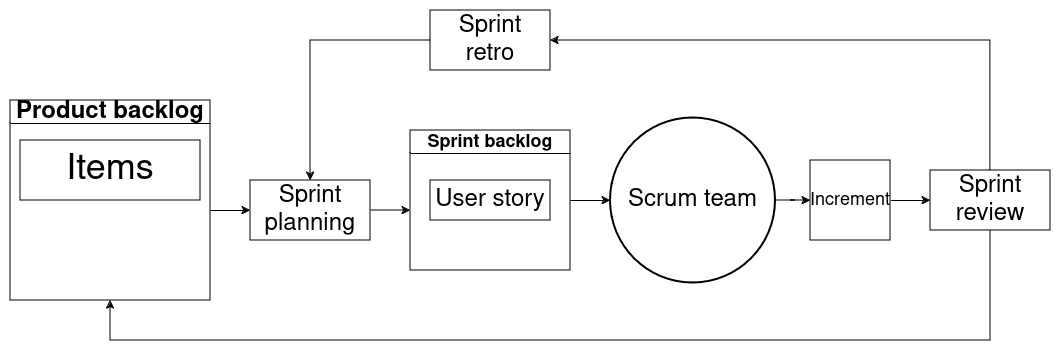
\includegraphics[width=\textwidth]{scrum.png}
\centering
\end{figure}

\subsection{Extreme programming}\label{xp}
Extreme programming is often more used in embedded domains where energy efficiency and performance have already been a concern for years due to hardware limitations~\cite{agilemethodsinembedded}. Extreme programming uses user stories to create a backlog like Scrum. Unlike Scrum, Extreme programming is more opinionated in how the actual development process is conducted. It enforces measures such as test-driven development, pair programming, enforced standards, and refactoring to ensure the quality of the software being produced. Extreme programming also imposes a 10-minute limit on build times for the software. In addition, extreme programming uses spikes which are simple throwaway programs to explore potential solutions to a complex or uncertain problem. The extreme programming process is illustrated in Figure~\ref{xpprocess}.~\cite{extremeprogrammingExtremeProgramming}

\begin{figure}[H]
\caption{Extreme programming project steps~\cite{extremeprogrammingFlowChart}}
\label{xpprocess}
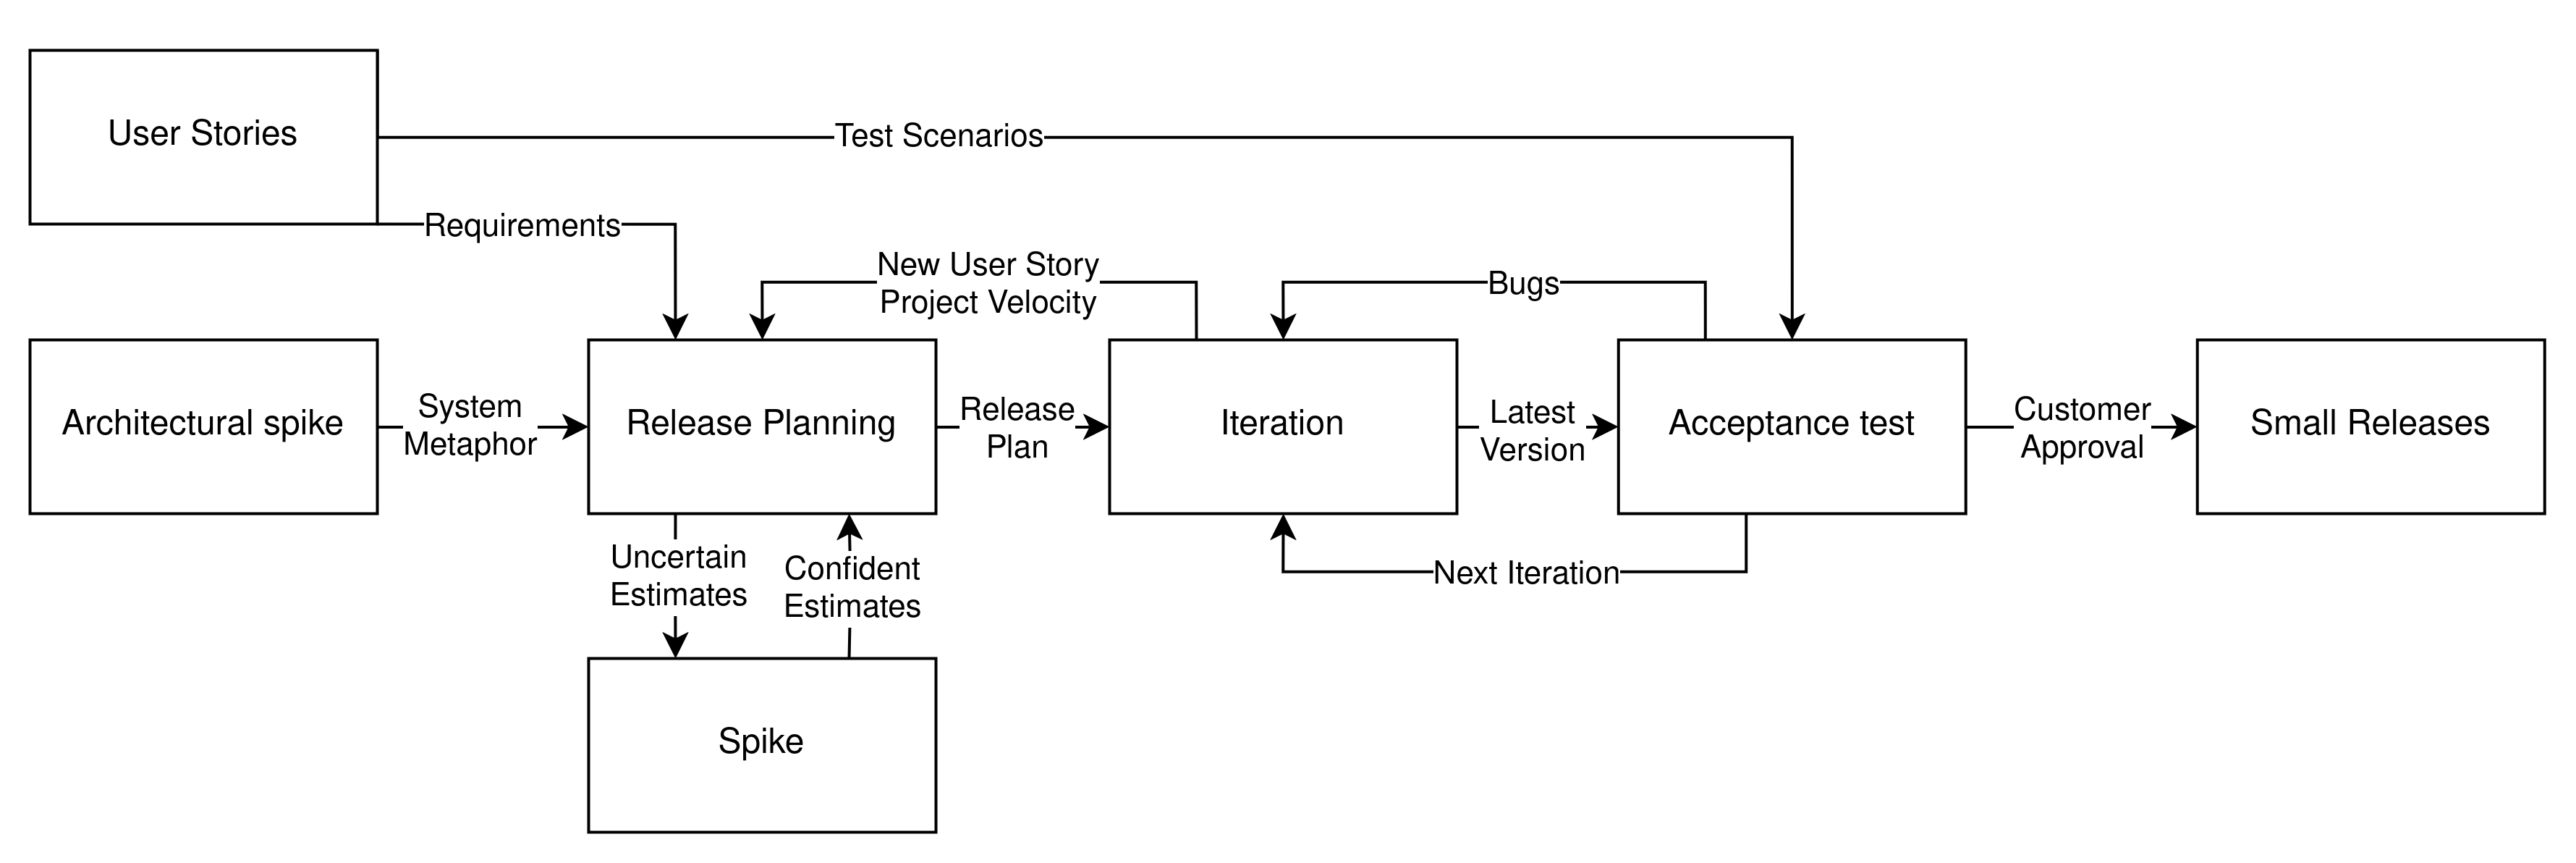
\includegraphics[width=\textwidth]{images/xp.png}
\centering
\end{figure}

\subsection{Kanban}\label{kanbanmethod}
Kanban is the simplest of the three most used Agile methodologies. Kanban can also refer to the Kanban board as a tool that is often used in other agile processes such as Scrum or Extreme programming. Kanban uses the Kanban board to keep track of the work. The Board is separated into different statuses of the tasks or user stories that are currently being done. Unlike Scrum, Kanban does not have specific roles for different members of the team. The Kanban board is shown in Figure \ref{kanban}.

\begin{figure}[H]
\caption{Kanban board}
\label{kanban}
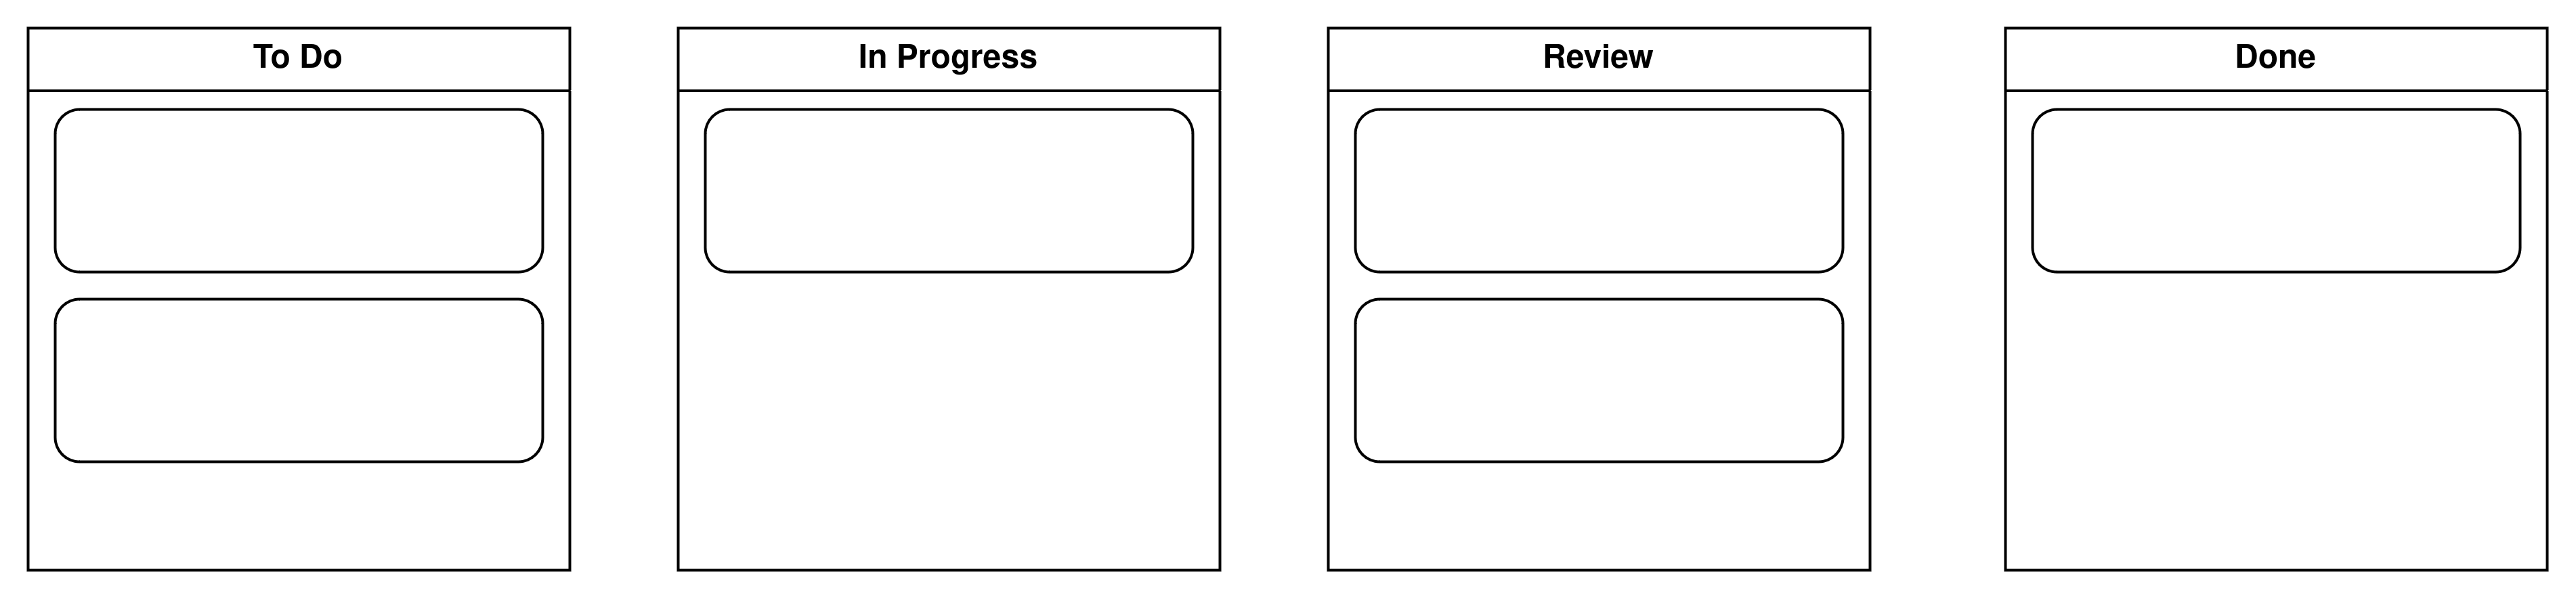
\includegraphics[width=\textwidth]{kanban}
\centering
\end{figure}

\section{Existing research for developing green software}
There is some existing research on developing software while taking into account its impact. This section explores three such development models.

\subsection{The Greensoft model}\label{greensoft}
The Greensoft model is a reference model for software engineering that takes into account the entire life cycle of a software product from development to end of life. It also presents metrics for measuring sustainability, procedures for different parties involved in the use of software, and tool recommendations for these parties. The overview of the Greensoft model is shown in Figure~\ref{greensoftoverview}.

\begin{figure}[H]
\caption{Overview of the Greensoft model~\cite{greensoft}}
\label{greensoftoverview}
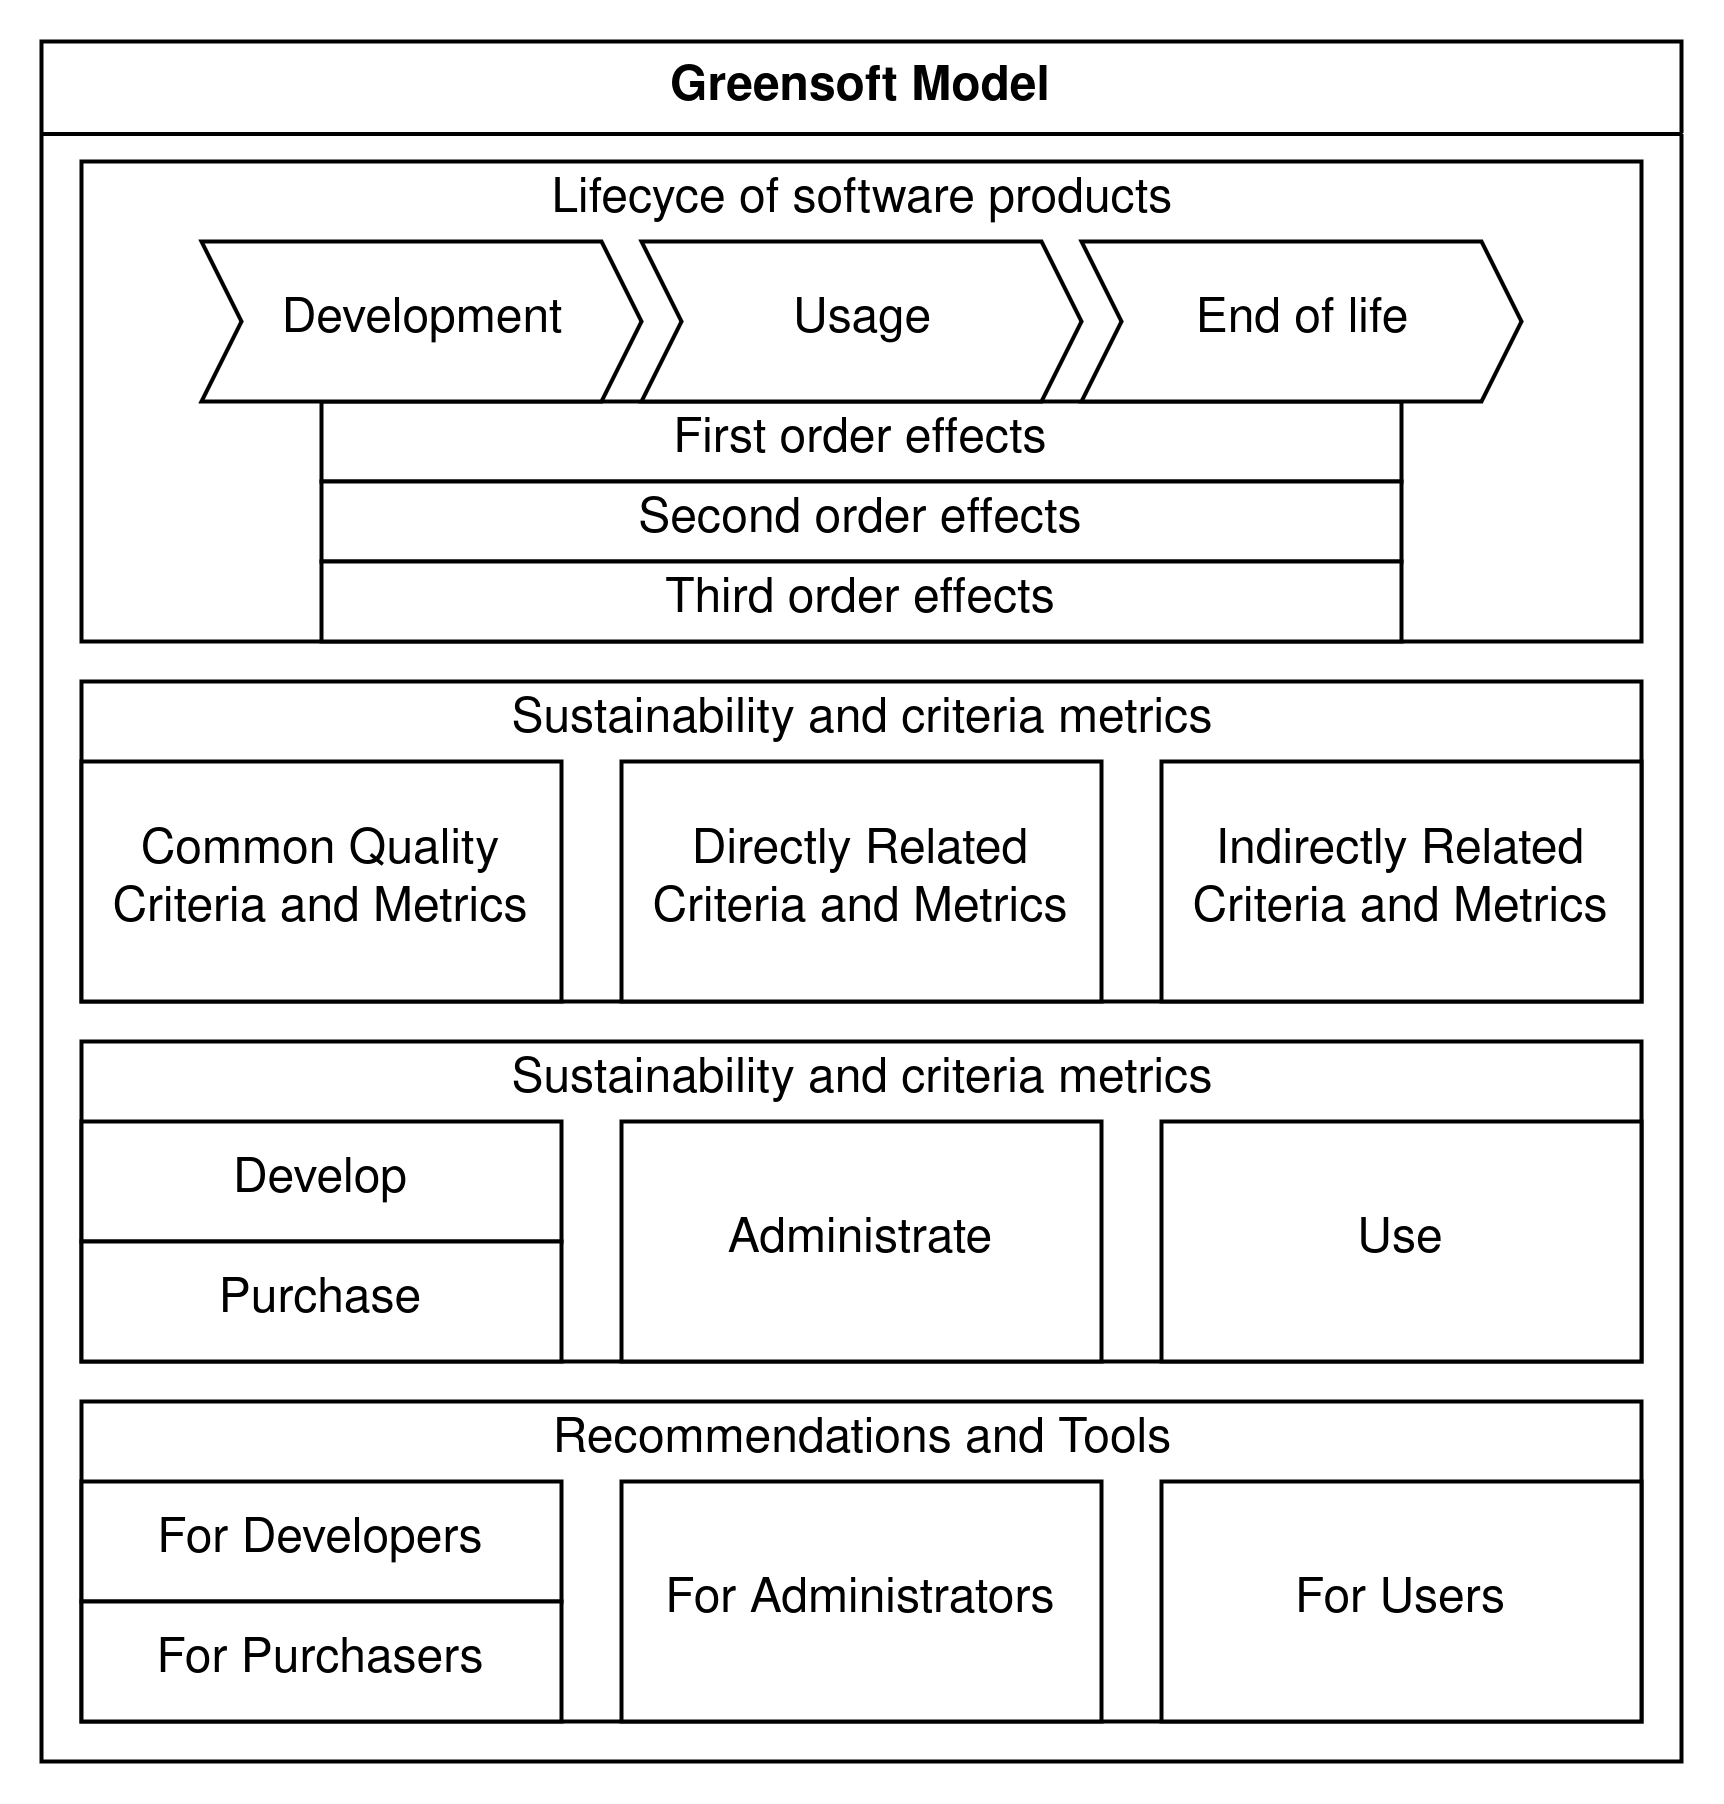
\includegraphics[width=\textwidth]{images/greensoft.png}
\centering
\end{figure}

\subsubsection{Life cycle of a software product}
The life cycle of software products is split into 3 different parts: development, usage, and end of life. All parts have first-, second-, and third-order effects on the sustainability of the software. First-order effects include direct effects of ICT supply. These include things such as performance and hardware requirements. Second-order effects include the effects of ICT usage. Third-order effects are the systemic effects of ICT. First-order effects are therefore in the \gls{greeninit}-category and second and third-order effects in \gls{greenbyit}- category~\cite{greensoft}. As this thesis is focused on the \gls{greeninit} category, first-order effects will be focused on here. The Life cycle of a software product is shown in Figure~\ref{lifecycle}.

\begin{figure}[H]
\caption{Life cycle of the software product}
\label{lifecycle}
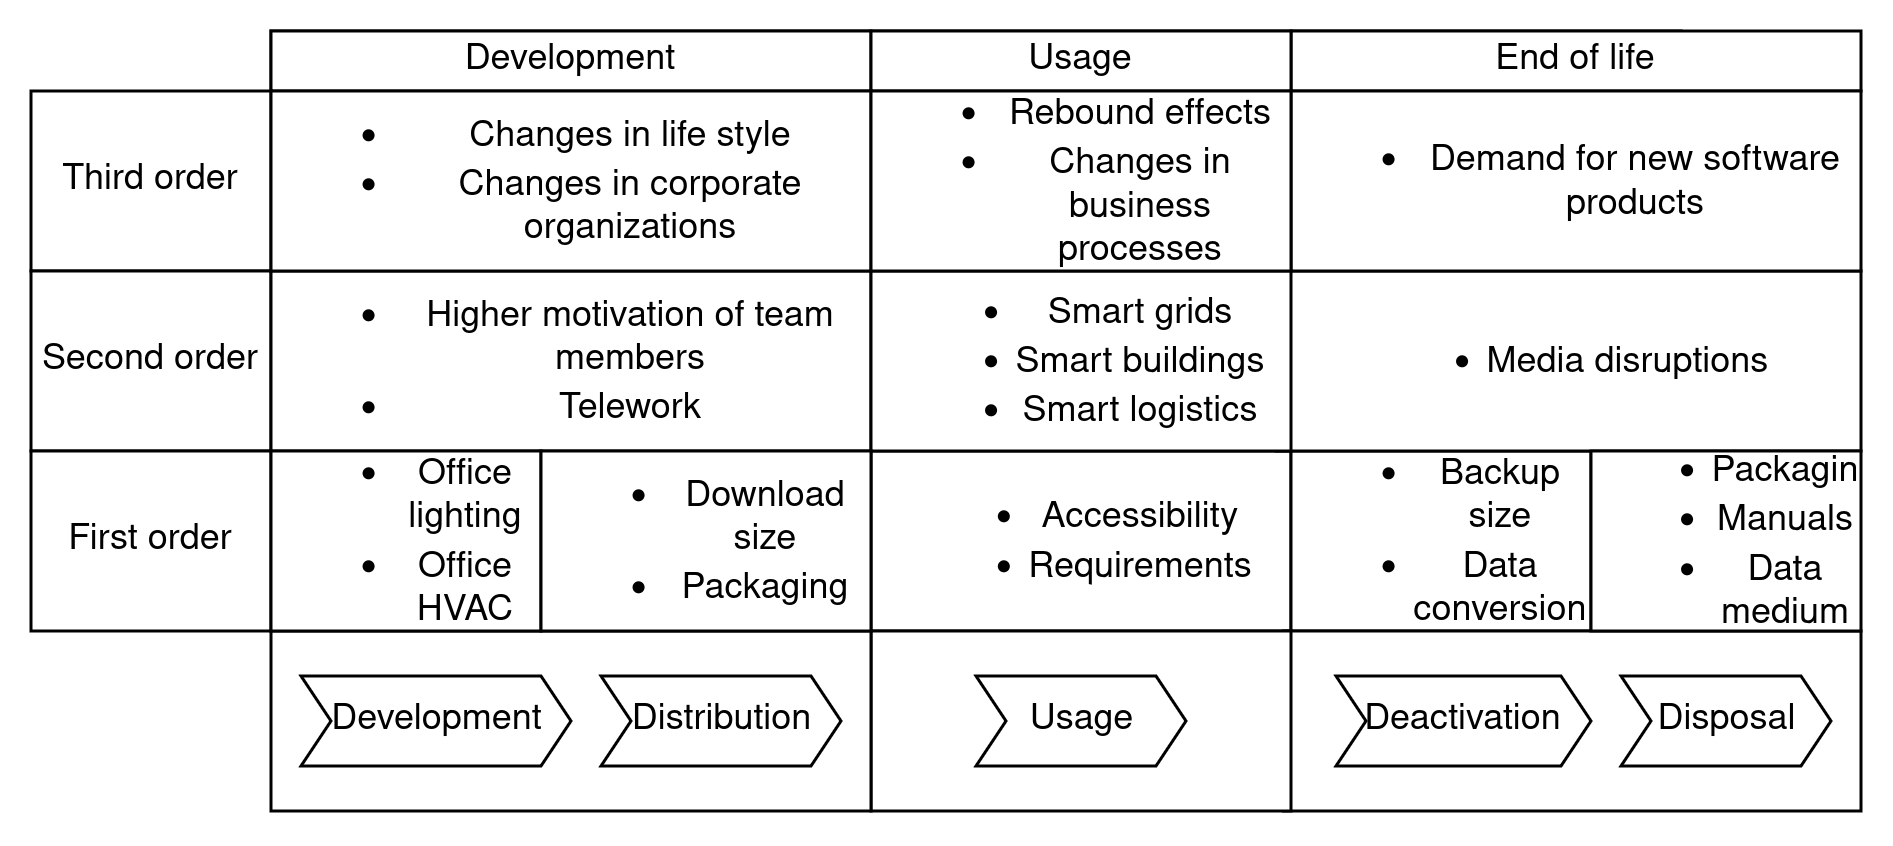
\includegraphics[width=\textwidth]{images/lifecycle.png}
\centering
\end{figure}

The development phase of the Greensoft model takes into account both development and distribution factors. These include office costs and conditions, commuting to work, business trips, and ICT energy usage. The distribution part includes things such as the size of the software, data formats, packaging, and transportation.

The usage part of the software is concerned with hardware requirements and overall energy consumption of the software and other resources required by it. The usage phase is the most affected by the software itself being as energy efficient as possible.

The final phase, end of life, is split into deactivation and disposal. Deactivation is concerned with preserving the data from the software and as such is affected by the backup size, format, and conversion of the data and long-term data storage. The disposal part on the other hand takes into account the data medium and packaging. This phase is used when at some point maintaining existing software can become too costly and a new software solution might be required. This can also be caused by changing business requirements or priorities. Energy consumption in this phase is mostly caused by saving and archiving data from the old software product because of legal restrictions or migrating data to the new software product. For these cases choosing the correct data format and compression method can make the migration easier and save time and disk space, which in turn reduces the energy needed.

\subsubsection{Indirect effects during development}
Some things affect the total energy use of the development that are not directly related to the software being made. These are called second and third-order effects~\cite{greensoft}. The office space used for working and how efficient it is regarding things such as heating and air conditioning are also factors. Some new building may even produce their energy with solar panels and be able to store it in batteries for later use. Indirect effects are mostly outside the scope of this thesis.

Remote working can also affect total energy consumption. Depending on the distance from home to the office and what is used to commute to work, it might be better to work remotely when possible and utilize different communication services to work in teams.

Development time and effects related to that should also be considered. The choice of the most efficient technologies might not be a net positive if developers are not familiar with them and developing the software takes longer than with familiar technologies.

Organizations can affect how people commute by providing public transportation tickets for workers or otherwise encouraging using public transport or non-polluting vehicles such as bicycles. The viability of these options is somewhat dependent on the distance between the workplace and the home of the employee.

\subsubsection{Sustainability Criteria and Metrics}
The model presents different quality properties that can be observed in different phases of the software lifecycle. The development phase lists modifiability, reusability, predictability, and efficiency as properties. Usage phase on the other hand lists portability, stability, performance, dependability, usability, and accessibility.

The model states that hardware lifetime should be maximized in order to prevent costs from replacing it. For this purpose the performance and portability of the software are important as performance helps maximize the lifetime of hardware and portability makes it easier to switch hardware when replacing it becomes necessary.

Energy efficiency is also an important metric. Energy efficiency is affected by more than just the runtime performance of the software. For example, lowering performance requirements or required service quality can help in reducing the overall energy usage of the software.~\cite{greensoft}

\subsubsection{Procedure models}
The procedure models presented in the model are split into develop, purchase, administrate, and use submodels.

The development model proposes adding sustainability review and preview, process assessment, sustainability journal, and sustainability retrospective to the software development process. The idea behind this is that these can be added to any software development process that is iterative.

The purchase model mostly focuses on procurement processes. Purchasing and procurement processes can define criteria that require measurement of energy efficiency, specific features such as those presented in the Criteria for software systems~\cite{kriteeripankkiSoftwareServices}.

The administrator model focuses on allowing administrators to install, configure, and monitor the software. This includes allowing administrators to check the energy and resource consumption of the software.

The use model focuses on how the users use the software. This is affected by the design of the software as well as the features in it that allow users to customize their experience. Displaying data on software resource usage and energy consumption may also affect the usage of the software by users.

\subsubsection{Recommendations and tools}
The model recommends making tools and recommendations available for different user groups to monitor and improve their energy usage. These tools and recommendations can include checklists, best practices, and guides for different user groups on how to use software more efficiently. This could be an optimization guide for developers, for administrators a tool that allows them to make infrastructure choices based on sustainability, and for users, a tool that allows them to configure their system's behavior regarding performance and energy consumption.~\cite{greensoft}

\subsection{A Green Model for Sustainable Software Engineering}\label{greenmodelforsustainable}
Mahmoud and Ahmad present a two-level model for creating green software and measuring the greenness of the software~\cite{greenmodelforsustainable}. The first level of the model aims to present an agile and green software development process. The second level presents different ways to measure the greenness of the software using existing tools and methods.

\subsubsection{Level 1}
The first level is divided into seven stages that represent different parts of the software engineering process. These stages are shown in Figure~\ref{level1}. 

\begin{figure}[H]
\caption{Level 1 of the green model for sustainable software engineering~\cite{greenmodelforsustainable}}
\label{level1}
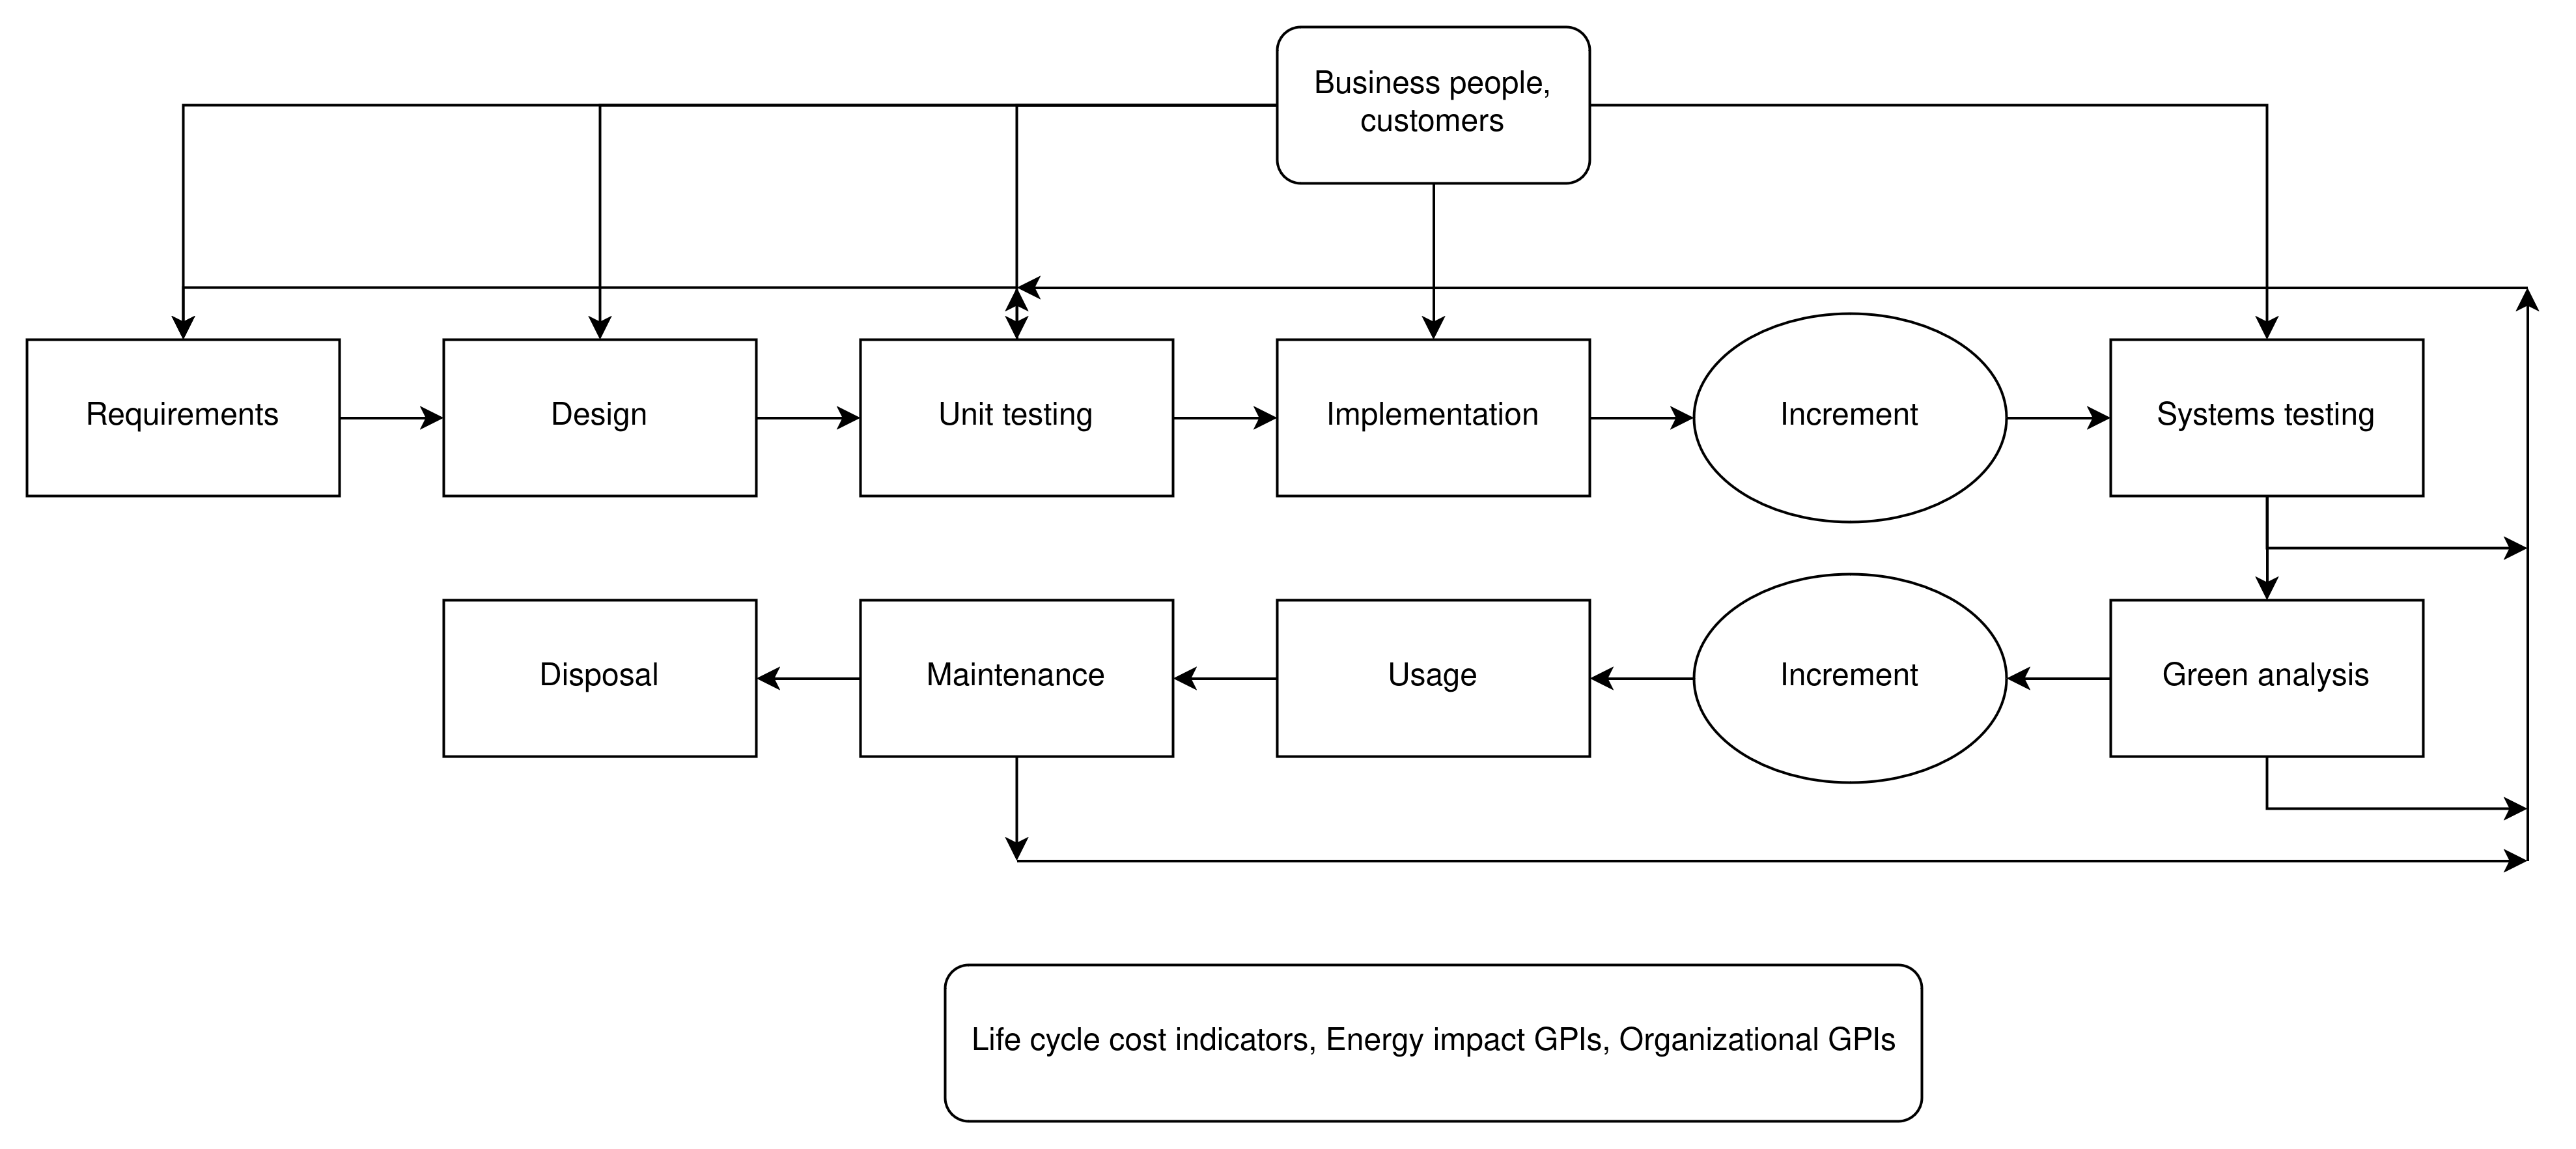
\includegraphics[width=\textwidth]{level1.png}
\centering
\end{figure}

The first stage is requirements engineering. This stage aims to determine the feasibility of the system if the system can solve the specific problem, create an outline for services to be provided, order the services, analyze the risk in terms of energy, and finally test the requirements. This stage is inspired by extreme programming conventions of requirements testing.

The design and implementation stages are used to create system architecture based on requirements. This stage includes guidelines for designing environmentally sustainable software. The guidelines mention using efficient algorithms based on the used data structures, programming languages, and hardware. The guidelines also mention that systems should stick to design and be as small as possible to avoid unnecessary lines of code. Frameworks and libraries are mentioned as potentially detrimental as they add more layers to software and might make it more inefficient.

The third stage is the testing stage which aims to discover defects in software functionality or meeting requirements. Tests should be developed early in the project. The paper presents metrics including fault tolerance, failure management, and testability for measuring the environmental impact of testing on software.

The fourth stage is analysis which aims to measure the energy usage of the software itself using metrics such as CPU usage, performance tests such as benchmarks and debug logs. Hardware may also support specific power measuring functions that could be used.

The fifth stage is usage which takes into account how users use the program. Software should aim to be simple and allow users to perform the minimum amount of actions for software to fulfill its purpose. Software should also support power management features such as using minimal power when idle.

The sixth stage is maintenance. This step is concerned with the maintainability of the software such as required access and knowledge to perform it and the amount and quality of documentation available for the software.

The final stage is disposal and it is concerned with how well the software can be recycled and reused in other software, how hardware can be recycled or repurposed, and how efficiently is migrating to the next software product.~\cite{greenmodelforsustainable}

\subsubsection{Level 2}
The second level introduces different tools for creating, measuring, and using energy-efficient software. This includes operating systems, application frameworks, energy usage measurement software, virtualization technologies for maximizing hardware use, and \gls{greenbyit} products that are used to help reduce energy consumption. The second level is shown in Figure~\ref{level2}.~\cite{greenmodelforsustainable}

\begin{figure}[H]
\caption{Level 2 of the green model for sustainable software engineering~\cite{greenmodelforsustainable}}
\label{level2}
\includegraphics[width=\textwidth]{level2.png}
\centering
\end{figure}

\subsubsection{Tools and Metrics}
The paper presents metrics for measuring the impact of the software being developed. These metrics are presented in Figure~\ref{metrics}. The GPI metrics are divided into IT resource usage, applications life cycle KPIs, Energy impact, and Organizational GPIs.

IT resource usage metrics take into account the resource usage of the software, Application lifecycle takes into account the development and configuring costs. The energy impact on the other hand takes into account the impact of data centers. The organizational GPIs include organizational factors. ~\cite{greenmodelforsustainable}

\begin{figure}[H]
\caption{Metrics for green software of the green model for sustainable software engineering~\cite{greenmodelforsustainable}}
\label{metrics}
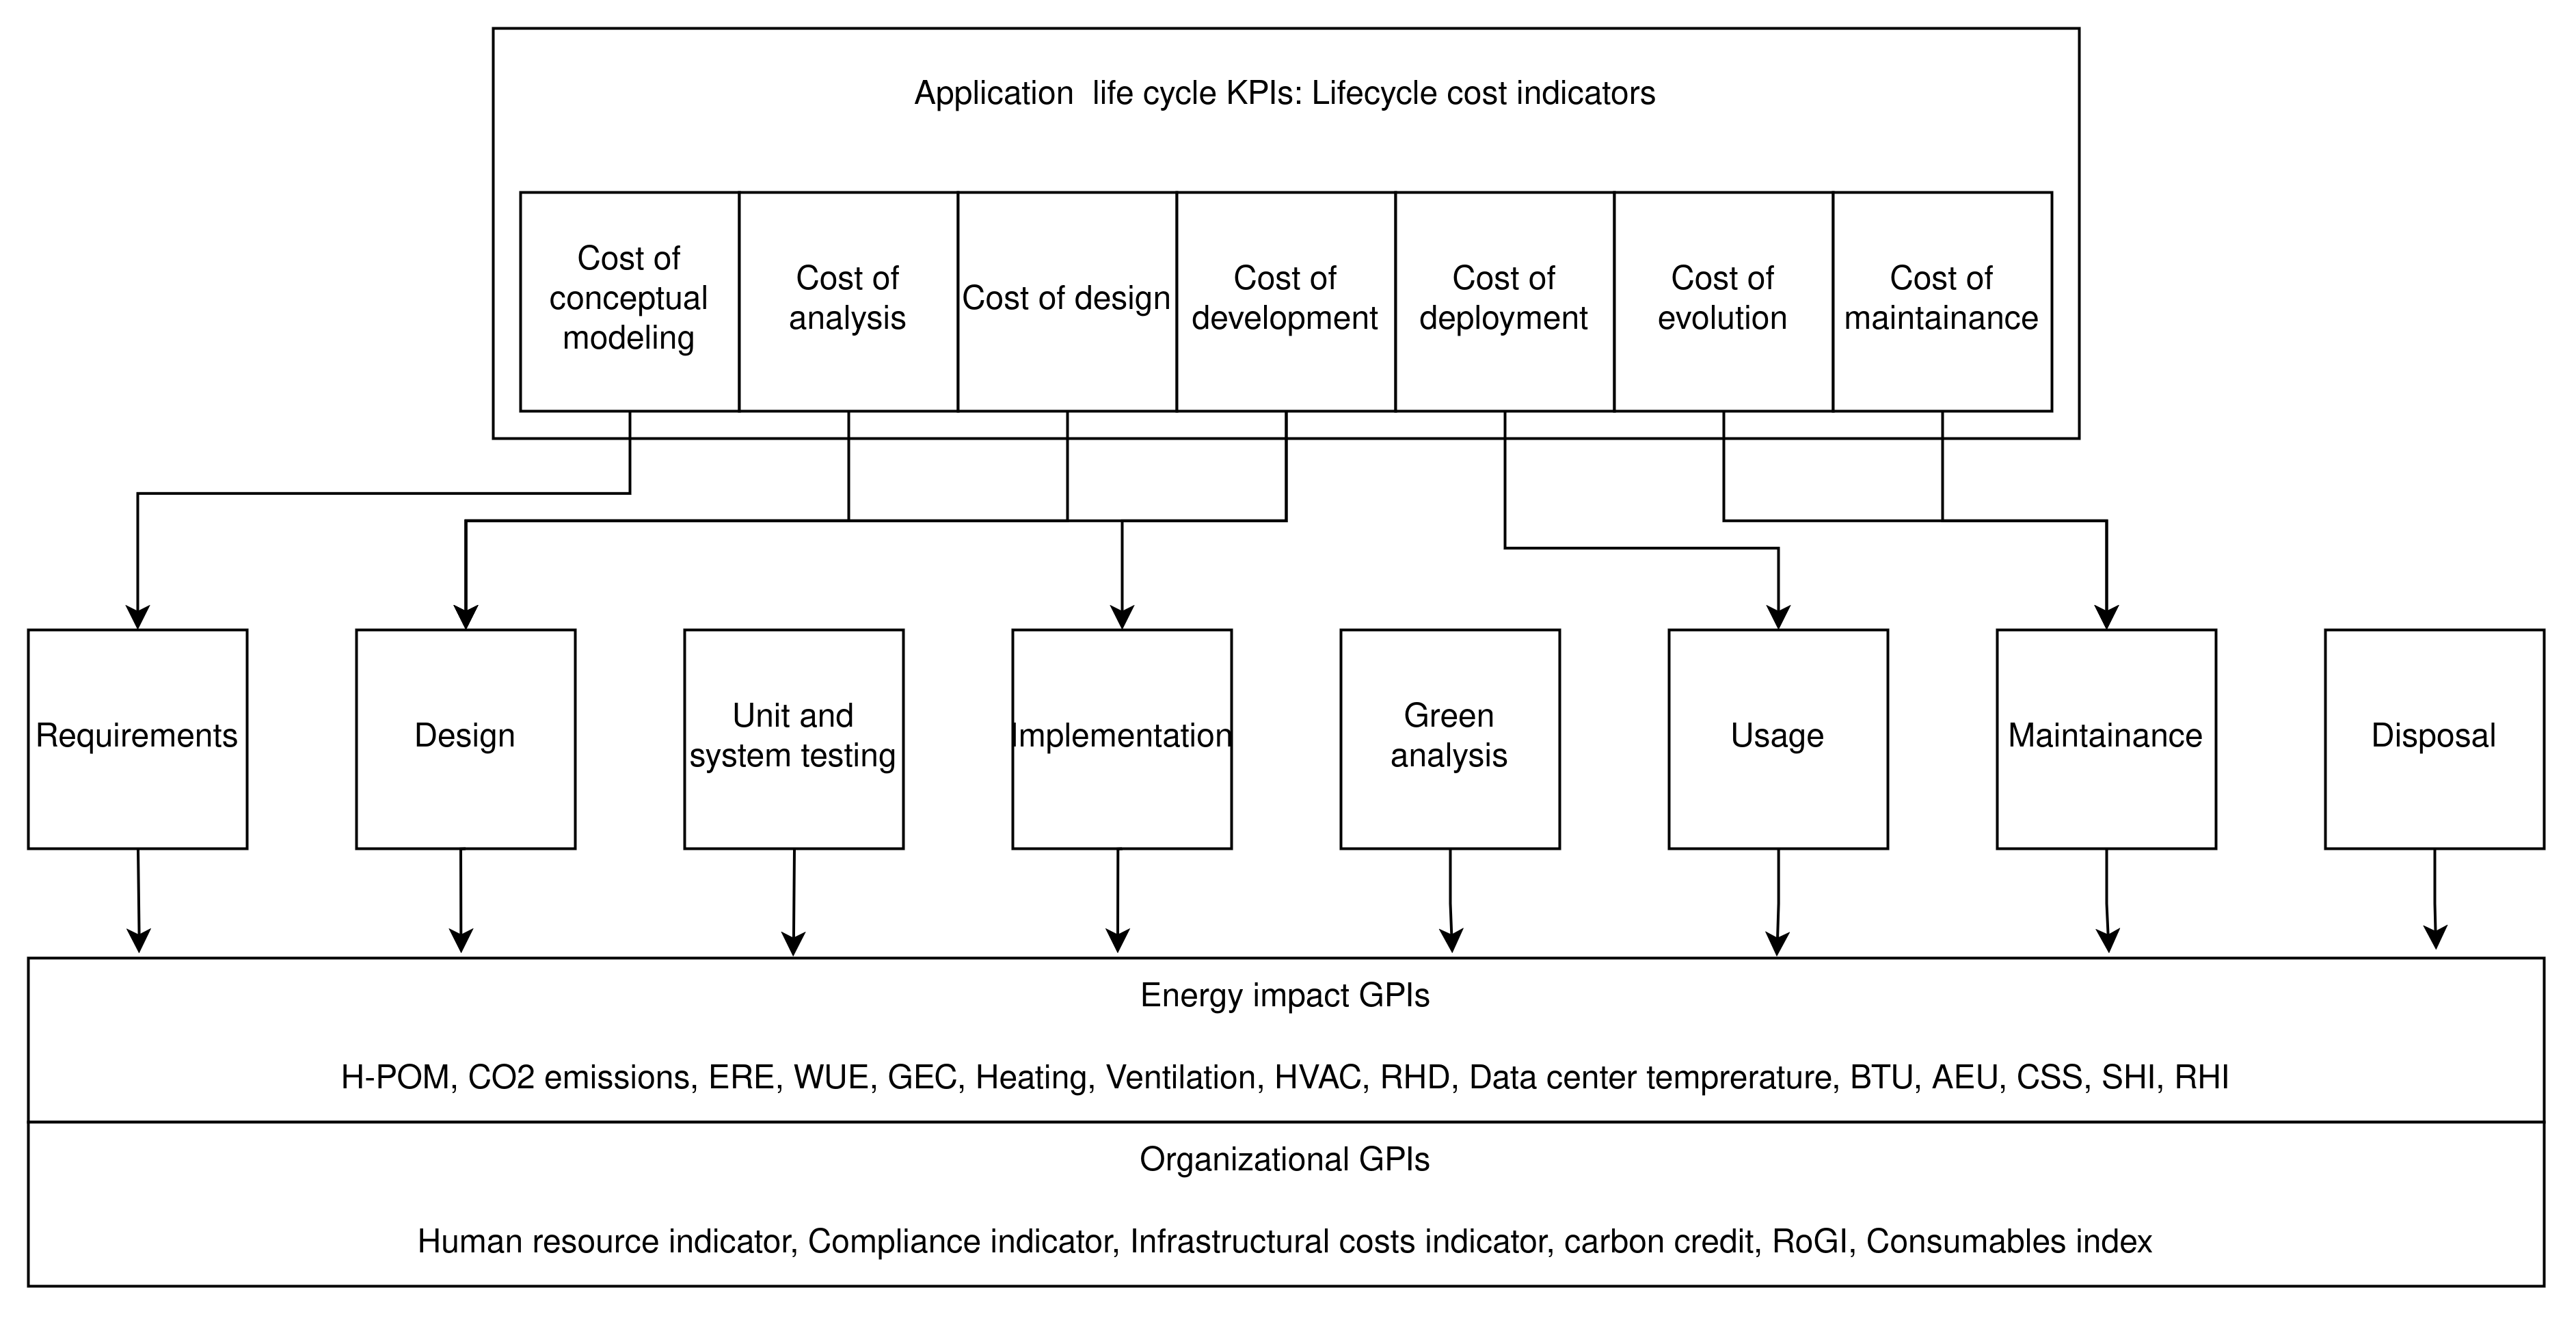
\includegraphics[width=\textwidth]{images/greenmetrics.png}
\centering
\end{figure}

\subsection{Green Lean process}\label{waste}
Ibrahim, Sallehudin, and Yahaya explore using lean methods to reduce waste in software development processes. It presents preliminary work for Green Lean Development components. The study considers Software waste, meaning incomplete work, unnecessary features, lost knowledge, hand-offs, task switching, delays, and defects, and theorizes that reducing them using lean methods will lead to greener software. Therefore sustainable software processes should strive to eliminate this waste. The paper shows that developing the Green Lean Model combines energy efficiency, waste reduction, and sustainable design~\cite{waste}. The process is shown in Figure~\ref{lean}.

\begin{figure}[H]
\caption{Green lean process~\cite{waste}}
\label{lean}
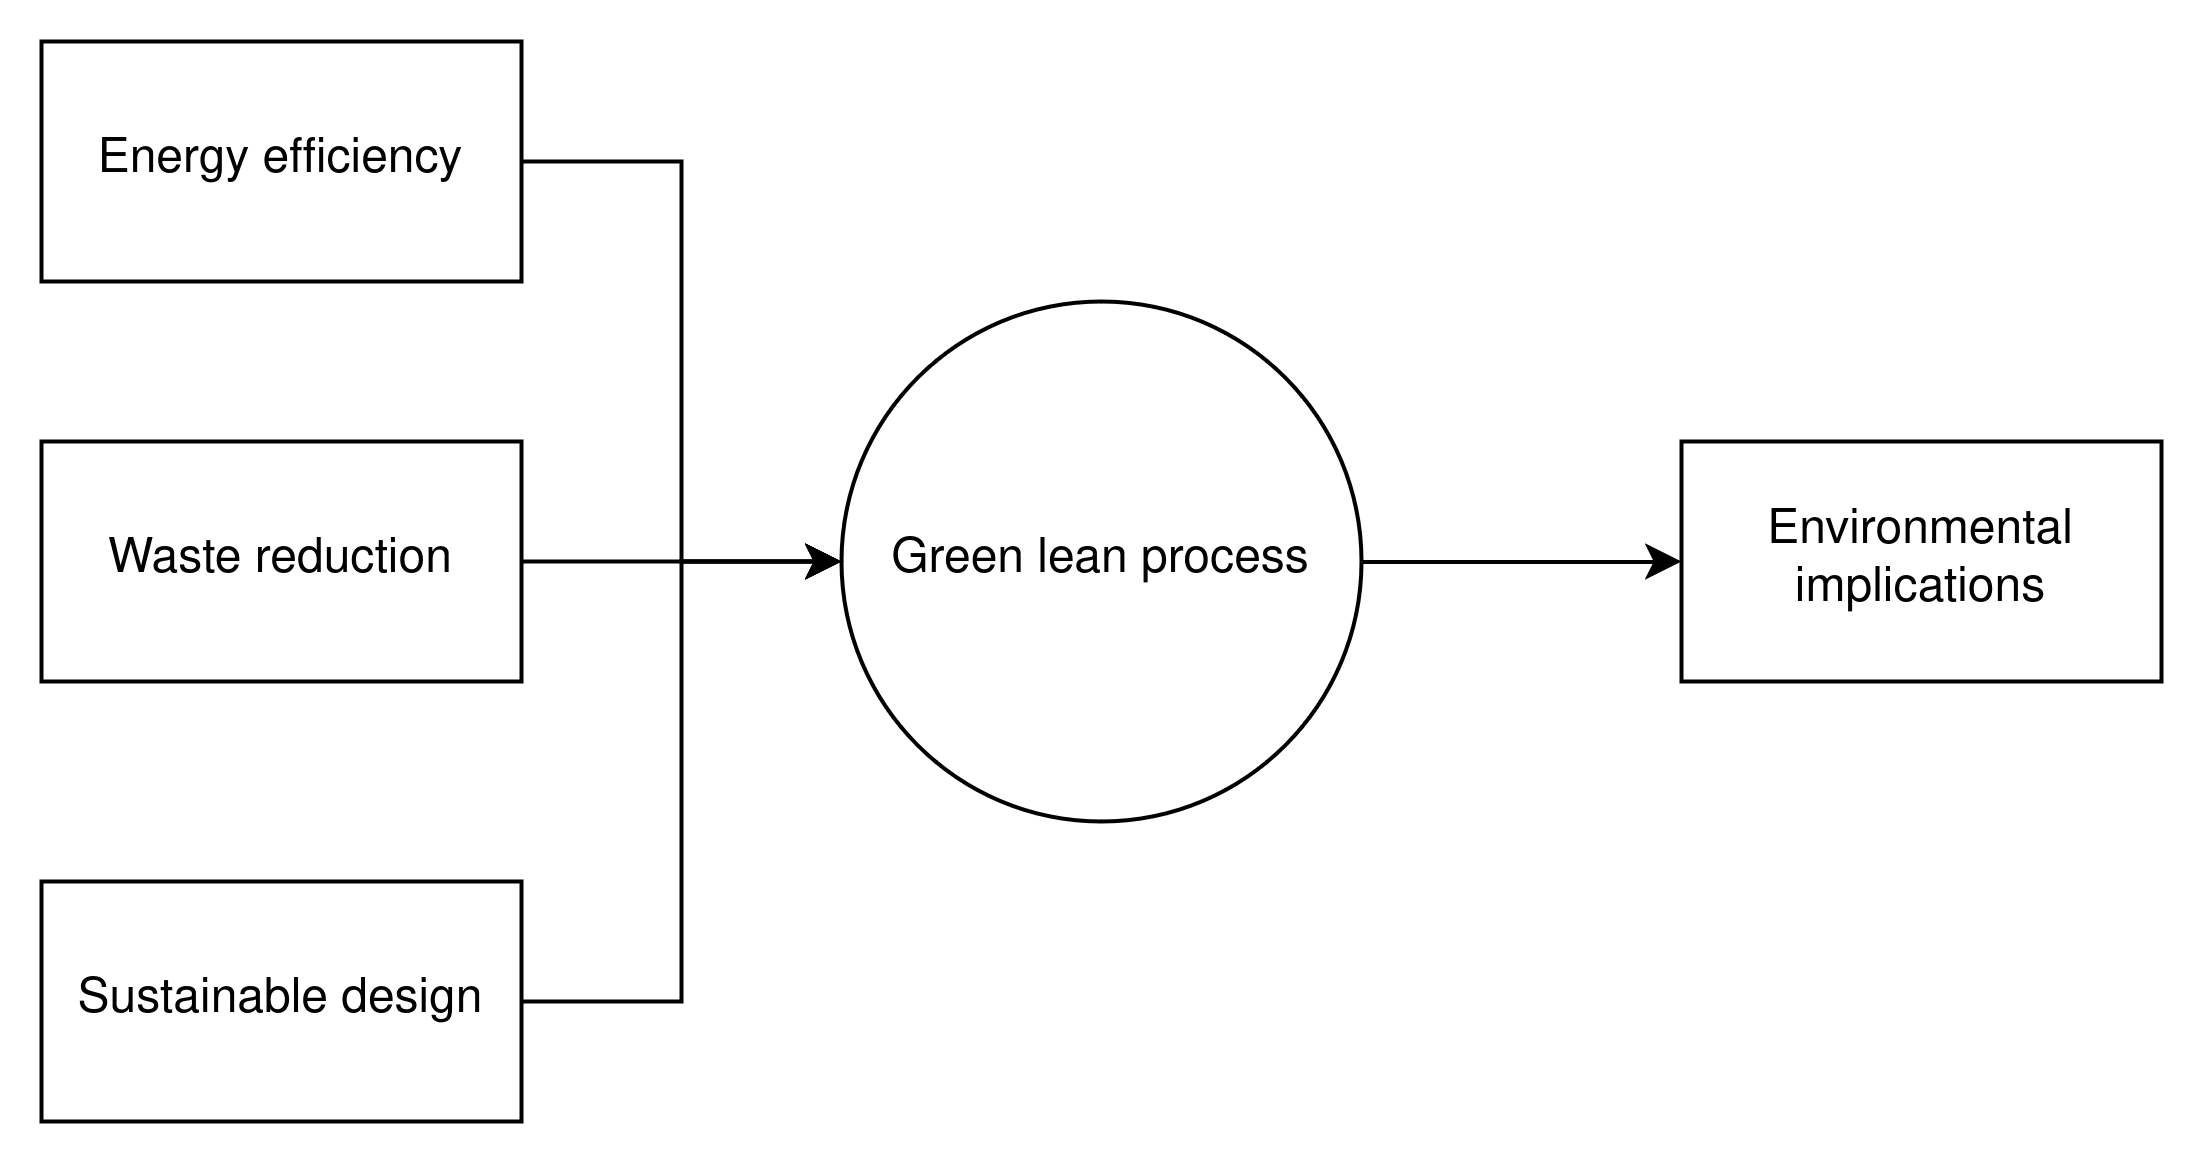
\includegraphics[width=\textwidth]{lean.png}
\centering
\end{figure}

\chapter{Measuring Sustainability of software}\label{chapter4}
Measuring the sustainability of software is critical for proving the benefits and improvements that can be made by optimizing software and its development process as well as helping guide decisions made during the development on what to focus on. This chapter answers \textbf{RQ2: How to measure the sustainability of the software?} by introducing metrics, methods, and tools for measuring different aspects of sustainability. 

\section{Metrics for Different Sustainability Aspects}\label{susmetrics}
There are many metrics to determine the sustainability of software and its development. The metrics should aim to measure different parts of sustainability such as technical, economic, environmental, social, and individual. As mentioned in Section~\ref{scope}, individual and social sustainability measurements are often outside the scope of single projects and should be measured on an organizational level and are therefore mostly outside the scope of this thesis.

\subsection{Technical Sustainability}
The \gls{technicalsustainability} of software should be measured to ensure the software being produced allows fast iterations and efficient solutions so no unnecessary work needs to be done to introduce new features or change existing ones. Technically sustainable software can also be more performant which affects both economic and environmental sustainability. To achieve \gls{technicalsustainability}, defects in software should be measured. This is usually done with project management tools where defects can be added to the development backlog and labeled.

In addition to defects, refactor opportunities should also be measured as they can tell if there is existing technical debt in the software being developed. Refactoring can be used to reduce technical debt and allow for faster iterations and feature additions.

Another measurement for \gls{technicalsustainability} is story points in user stories. This is used in many agile implementations to indicate the work required for a specific story. If completed story points are decreasing every sprint, it can indicate that technical debt is accumulating and slowing down development.

Crashes caused by unhandled errors should also be measured as they can indicate low stability of the software. Stability was one of the metrics identified in the Greensoft model in Section~\ref{greensoft}.

\subsection{Economic Sustainability}
For software to be sustainable, the costs of developing and using it should be measured. This is usually relatively easy when using hosting platforms or cloud service providers as they report the costs of running the software. In addition, the cost of the development team and tools used by them such as development tools and CI/CD pipeline usage costs should be measured to keep track of overall costs. These metrics include most of the lifecycle cost indicators presented in the green model for sustainable software engineering in Section~\ref{greenmodelforsustainable}. Cost of development was also mentioned as a relevant metric in the Greensoft model in Section~\ref{greensoft} as the "efficiency" metric.

\subsection{Environmental Sustainability}
As mentioned in Section~\ref{challenges}, the lack of tools is highlighted as one of the biggest challenges in measuring the energy consumption of software which presents challenges for measuring the \gls{environmentalsustainability}.

Studies on measuring energy efficiency show that energy, performance, utilization, and economic, performance in relation to energy and pollution are used as metrics~\cite{slronmetrics}. Findings of Section~\ref{methods} support performance as a good heuristic for energy consumption. This applies to energy in relation to performance as well. This means that during development, benchmarks can be used to measure the \gls{environmentalsustainability} of specific features or code paths. In addition, benchmarks can catch regressions in software that affect \gls{environmentalsustainability} and by extension \gls{economicalsustainability}. Performance was also included as a key metric in the Greensoft model in Section~\ref{greensoft}.

Resource utilization can reveal high network or disk (I/O) usage which can be mitigated with caching strategies and architectural improvements. High CPU usage can also be a good or a bad thing depending on the performance achieved. It can mean that the application is busy waiting instead of allowing other tasks to use the CPU time but it can also mean that the system resources are utilized well. Measuring resource utilization can therefore reveal good refactoring opportunities.

Depending on the platform the software is running on, resource usage and energy consumption can be read directly from the operating system using APIs such as \gls{rapl} and reported as part of the telemetry and logs collected such as in native desktop or mobile applications. On servers, different tools can be installed to monitor and report energy consumption and resource usage. Cloud service providers also allow monitoring of resource usage and sometimes even metrics directly relevant to \gls{environmentalsustainability} such as CO2 emissions or energy usage.

\section{Measurement Tools}\label{tools}
There are many tools available for measuring different aspects of sustainability. Project management tools often allow measuring the number of items such as user stories, velocity of development by assigning story points to items, and costs relating to development. For \gls{environmentalsustainability} there exist tools for measuring resource usage and energy consumption for different hosting infrastructures.

\subsection{Technical Sustainability}
Defects and refactor opportunities can be measured with project management tools such as Kanban boards. Most kanban board tools allow labeling items or events separating them into different lanes or boards. These tools often also report the number of items on each label or board.

\subsection{Economical Sustainability}
Cost of development is often measured using work time tracking, project billing per hour or per month, and costs reported by development tools such as CI/CD pipeline and hosting costs. These should be collected and available to customers and the development team.

\subsection{Environmental Sustainability}
There are different tools for measuring software energy consumption. Measuring tools can be broadly separated into three different categories: Software tools, Hardware devices, and hybrid methods~\cite{8716456}. The software tools are generally not as accurate but they are more convenient and easily available as software is often run in cloud environments and having a physical testbench on premises is not always possible.

\subsubsection{Software Tools}
Software tools can be used to estimate the energy consumption of the system or processes based on available hardware sensors in different components of a computer and are as such limited to what sensors hardware offers. In addition to these methods, benchmarking software performance and resource usage can give some indication of its energy usage characteristics and can be used to detect changes in energy usage during the program lifecycle. Most software tools are based on \gls{rapl} API and \gls{msr}s. These have been proven to be accurate measurements of energy usage and therefore software tools based on them can be used to give at least a fairly accurate estimate of energy usage~\cite{shortcodepathrapl}\cite{raplinaction}. The overhead from RAPL is also negligible~\cite{raplinaction} and should not affect the measurements.

Profiling and monitoring tools can be used to determine the energy consumption of processes. In some cases, profiling tools can introduce overhead which affects the overall performance of the program and can make them unsuitable for production usage~\cite{profilingenergyprofilers}\cite{calmenergyaccounting}. Some tools such as JoularJx can be used to measure the energy consumption of specific methods but might be limited in their programming language support~\cite{joularjx}.

Monitoring tools such as PowerAPI~\cite{powerapi}, Schapandre~\cite{scaphandre}, PowerJoular~\cite{joularjx} and Green metrics tool~\cite{greenmetricstool} can be installed on the machine running the software such as on a server to continuously monitor the energy usage. Tools such as these do have their limitations, they might not work in virtualized environments unless the host has installed the software and exports metrics to virtualized guest systems. There are also many tools presented as an example in literature such as GreenTracker~\cite{greentracker} but finding working versions of these tools for general use is difficult.

Some tools can analyze the website on a given URL and give it a score based on several factors relating to greenness and efficiency. These tools can be used to evaluate front-end web applications. These tools are by themselves not enough but can be used to indicate potential optimizations for front-end applications. Google's lighthouse is one such tool. These tools should be also integrated into CI/CD pipelines if they provide an API that allows developers to do so or are usable locally such as Lighthouse.

\subsubsection{Hardware devices}
Power meters can be used to directly measure how much energy a computer is using while running software. This method must take into account all different services and operating systems running on a computer and first form a baseline idle energy consumption that is used when comparing to energy usage while a program to be measured is running~\cite{studyoninfluence}. Hardware tools are not always feasible for software development organizations and therefore for the model proposed by this thesis, software-based tools are recommended.
\chapter{Adapting Sustainable Agile for Kvanttori Case}\label{chapter5}
This chapter explores how agile software development is currently implemented at Kvanttori, what Kvanttori wants to achieve with a sustainable agile model, how to create and implement such a model, and how it differs from the current agile model at Kvanttori. This chapter answers \textbf{RQ3: How to integrate sustainable development methods into an agile development process?} by adding methods and criteria in Chapter~\ref{chapter2}, parts of different agile models in Chapter~\ref{chapter3}, and metrics and tools in Chapter~\ref{chapter4} to the current development model at Kvanttori.

\section{How Kvanttori Implements Agile}\label{currentimplementation}
The development model described in this section was created by gathering information from Kvanttori's internal development guides and by personally having worked on different projects at Kvanttori.

Kvanttori's current agile implementation is based on Scrum using Essential Scrum~\cite{essentialscrum} as a guidebook for applying Scrum during the development process. The process implements all parts of the Scrum framework as pictured in Figure~\ref{scrumprocess} in Section~\ref{scrum} as well as some additional parts from the Essential Scrum book. The current process is illustrated in Figure~\ref{kvanttoriagile}. The process is split into four sections: pre-development, development, usage, and post-development. Usually, the project starts with pre-development with development and usage happening at the same time when the project is in active development. Post-development phase happens after the project ends or moves into maintenance mode. The maintenance usually entails working on bug fixes and updating dependencies when needed. It can also include monitoring and fixing issues with the hosting environment as needed. Earlier phases can be revisited as necessary. Introducing a new feature might require new technologies to be evaluated and projects can return from maintenance to active development.

Currently, the development process does not take performance and other factors correlating with \gls{environmentalsustainability} into account as long as they are not part of the customer requirements. Only if some features must happen in a specific time limit or if performance is detrimental to usability, will it be used as a reason to not accept a feature as done. \Gls{economicalsustainability} is mostly the responsibility of the customer in the current model as costs are reported directly to the customer but following them and actively minimizing them is not prioritized over other tasks as long as they stay within the customer's budget. \Gls{technicalsustainability} is measured in the backlog using labels for defects in software but bugfixes and refactors are not systematically prioritized and can often stay in the backlog for a long time if not deemed critical.

\begin{figure}[H]
\caption{Kvanttori's current agile implementation}
\label{kvanttoriagile}
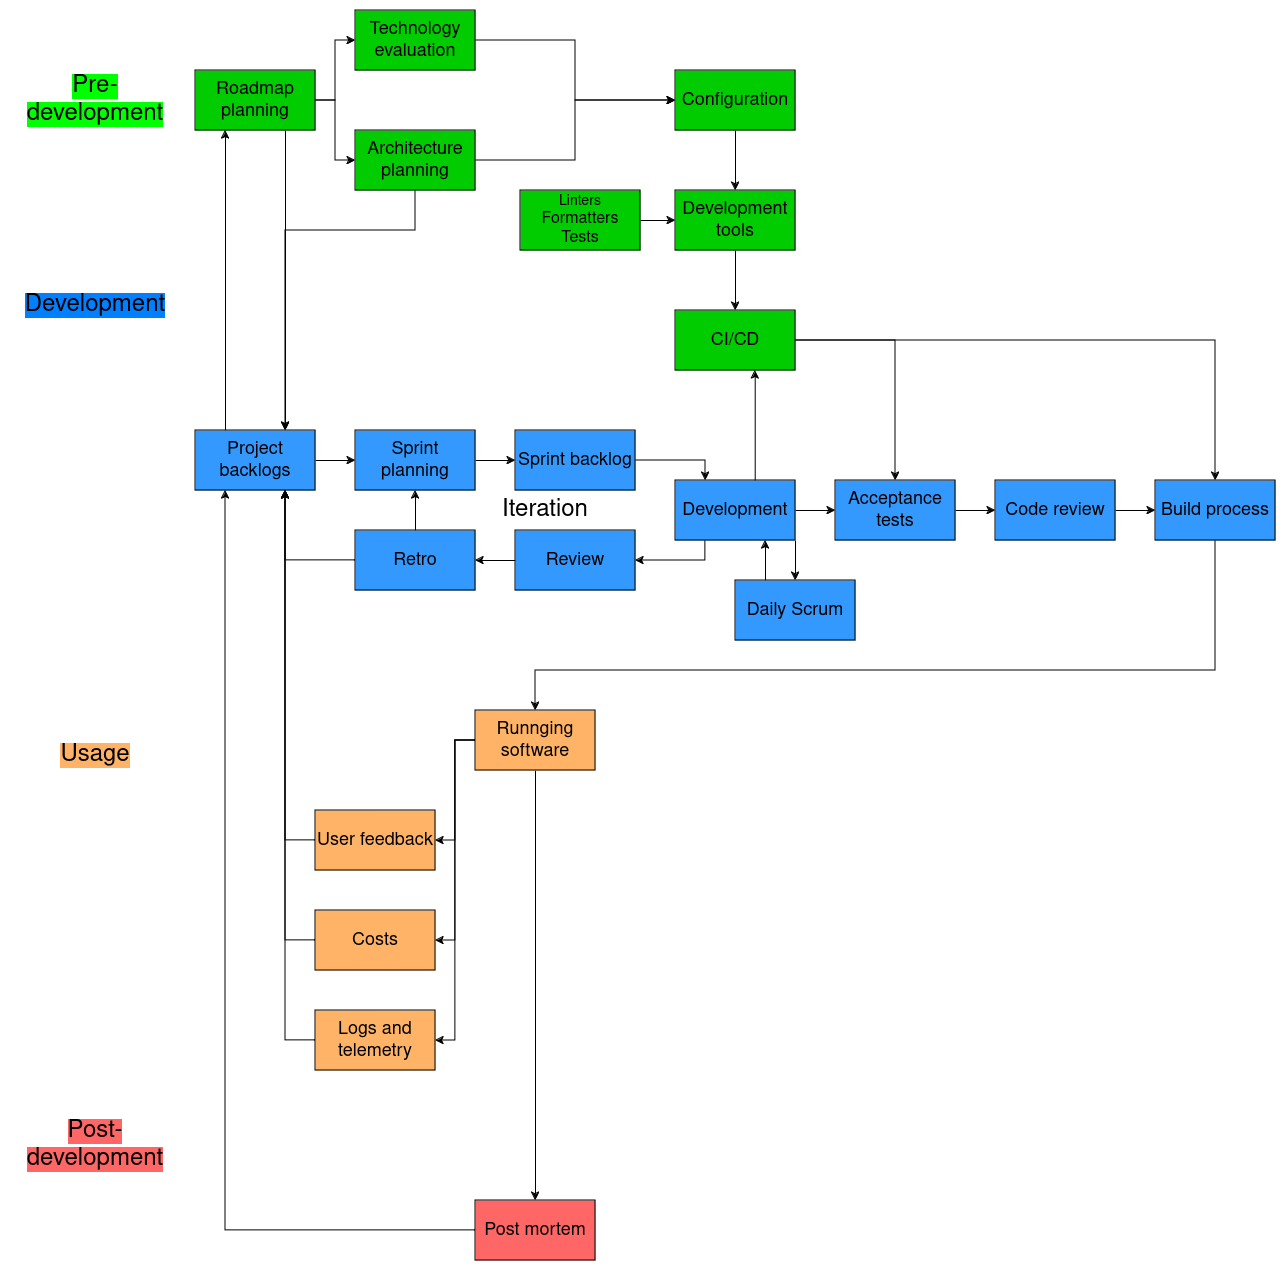
\includegraphics[width=\textwidth]{images/currentagile.png}
\centering
\end{figure}

\subsection{Pre-development Phase}
Pre-development phase consists of setting up the project, finding out high-level requirements, choosing technologies, and setting up the development environment.

\subsubsection{Roadmapping}
Projects start by meeting with a customer to get a better understanding of the customer's business and the problem that needs to be solved. During these meetings, high-level requirements are gathered for the software solution to be developed during the project. This entails estimating how many sprints there will be, how long they are, deadlines imposed by the customer, how releases are done, and estimated work required for the most central features. This is expected to change during the development process but it is used as a starting point for determining what big features are the most important. These features or epics will be split into smaller stories during development. This implements envisioning and release planning from the Essential Scrum~\cite{essentialscrum}.

\subsubsection{Technology Evaluation}
Technologies for a project are chosen based on customer and technical requirements such as previous technology used, platform support, and library ecosystem. The familiarity of the development team with technologies is also considered.

\subsubsection{Architectural Planning}
Architectural planning takes into account any customer requirements for existing systems interoperability with the software being developed as well as the needs of the software being developed.

Architectural planning also includes the distribution and hosting of the software. The choice of hosting methods and hosting provider is affected by the customer's existing systems, the need for scalability, costs, and the skill set of the development team.

\subsubsection{Configuration, Development Tools and CI/CD}
The configuring step is for setting up the necessary development tools and CI/CD pipelines for automated testing and releases.

All projects use linters, formatters, and testing tools to ensure the quality and readability of the code and to ensure the software is working as expected. These are chosen by the lead developer depending on the project and technologies used and are often integrated directly into the development environment as well as CI/CD pipelines.

\subsection{Development Phase}
The day-to-day development process follows Scrum closely including daily Scrum, sprint planning, retro and review steps. Kvanttori uses story points and planning poker together with project management tools to estimate and track team velocity.

Project backlogs are used to keep track of work to be done for the project. This is implemented with a Kanban~\ref{kanbanmethod} board that allows labeling use of stories with labels such as features or bugs.

Sprint planning is used to estimate story points and choose stories from the project backlog to the sprint backlog. The chosen stories depend on the stakeholder requirements as well as the amount of points assigned to each task.

Sprint backlog tracks work that needs to be done in the current sprint. This is implemented with the same tool as the project backlog.

Acceptance tests are automatically run in CI/CD pipelines to ensure compliance with formatting, linting, and tests.

Code review is conducted by other team members, often by the lead developer to ensure the quality of implementation and compliance with high-level architecture.

\subsection{Usage Phase}
Logs are collected from the software to find errors that users may run into and add fixing them to the product backlog. Telemetry may also be implemented to find what features are used the most but is not required.

\subsection{Post-development Phase}
Lastly, after the project ends, there is a post-mortem of the project where things learned from the project are discussed among the development team and written for other development teams to read for future projects.

\subsection{Roles}
Kvanttori has four roles in the development team with one person sometimes having multiple roles. These are Product owner, Scrum master, lead developer, and developer. With one person often taking on multiple roles due to team sizes. For example, the Product owner can also be the lead developer and the Scrum master is often also a developer. The lead developer is a role that is not specified in Scrum roles but has been deemed useful at Kvanttori based on experiences in different projects.

\section{Sustainable Agile Implementation}\label{susimplementation}
The sustainable agile model described in this section was created by implementing findings of the literature review including methods for creating sustainable software in Chapter~\ref{chapter2}, existing agile and sustainable agile methods in Chapter~\ref{chapter3}, and metrics and measurement tools in Chapter~\ref{chapter4} into the current development model used at Kvanttori presented in Section~\ref{currentimplementation}.

Kvanttori wants a model that allows it to create software that is more sustainable technically, economically, and also environmentally. The model should also aim to prevent the accumulation of \gls{sustainabilitydebt}~\cite{sustainabilitydebt} including technical sustainability debt, economical sustainability debt, and environmental sustainability debt. In addition, the model helps standardize the development model to ensure that teams have a checklist of issues to take into account in every project. This model should aim to include all methods for improving the sustainability of software presented in Section~\ref{methods} as well as issues raised in Chapter~\ref{chapter3} green agile models such as measuring and reporting sustainability, reducing waste in software and allow users to use software in more sustainable ways. The model should also implement metrics discussed in Section~\ref{susmetrics}. The result of using the proposed model should be software that is cheaper to develop and run, uses less energy, is faster, and is easier to maintain.

The new model retains the four phases of the current model, those being pre-development, development, usage, and post-development. Similarly to the current model, these phases can be revisited multiple times during development.

Some new steps and metrics for the development model are required to ensure that sustainability is taken into account during all phases of the development model. In addition, some existing steps and roles have been changed to better take sustainability into account. Figure~\ref{greenagile} illustrates the proposed process model.

\begin{figure}[H]
\caption{Proposed sustainable agile implementation model}
\label{greenagile}
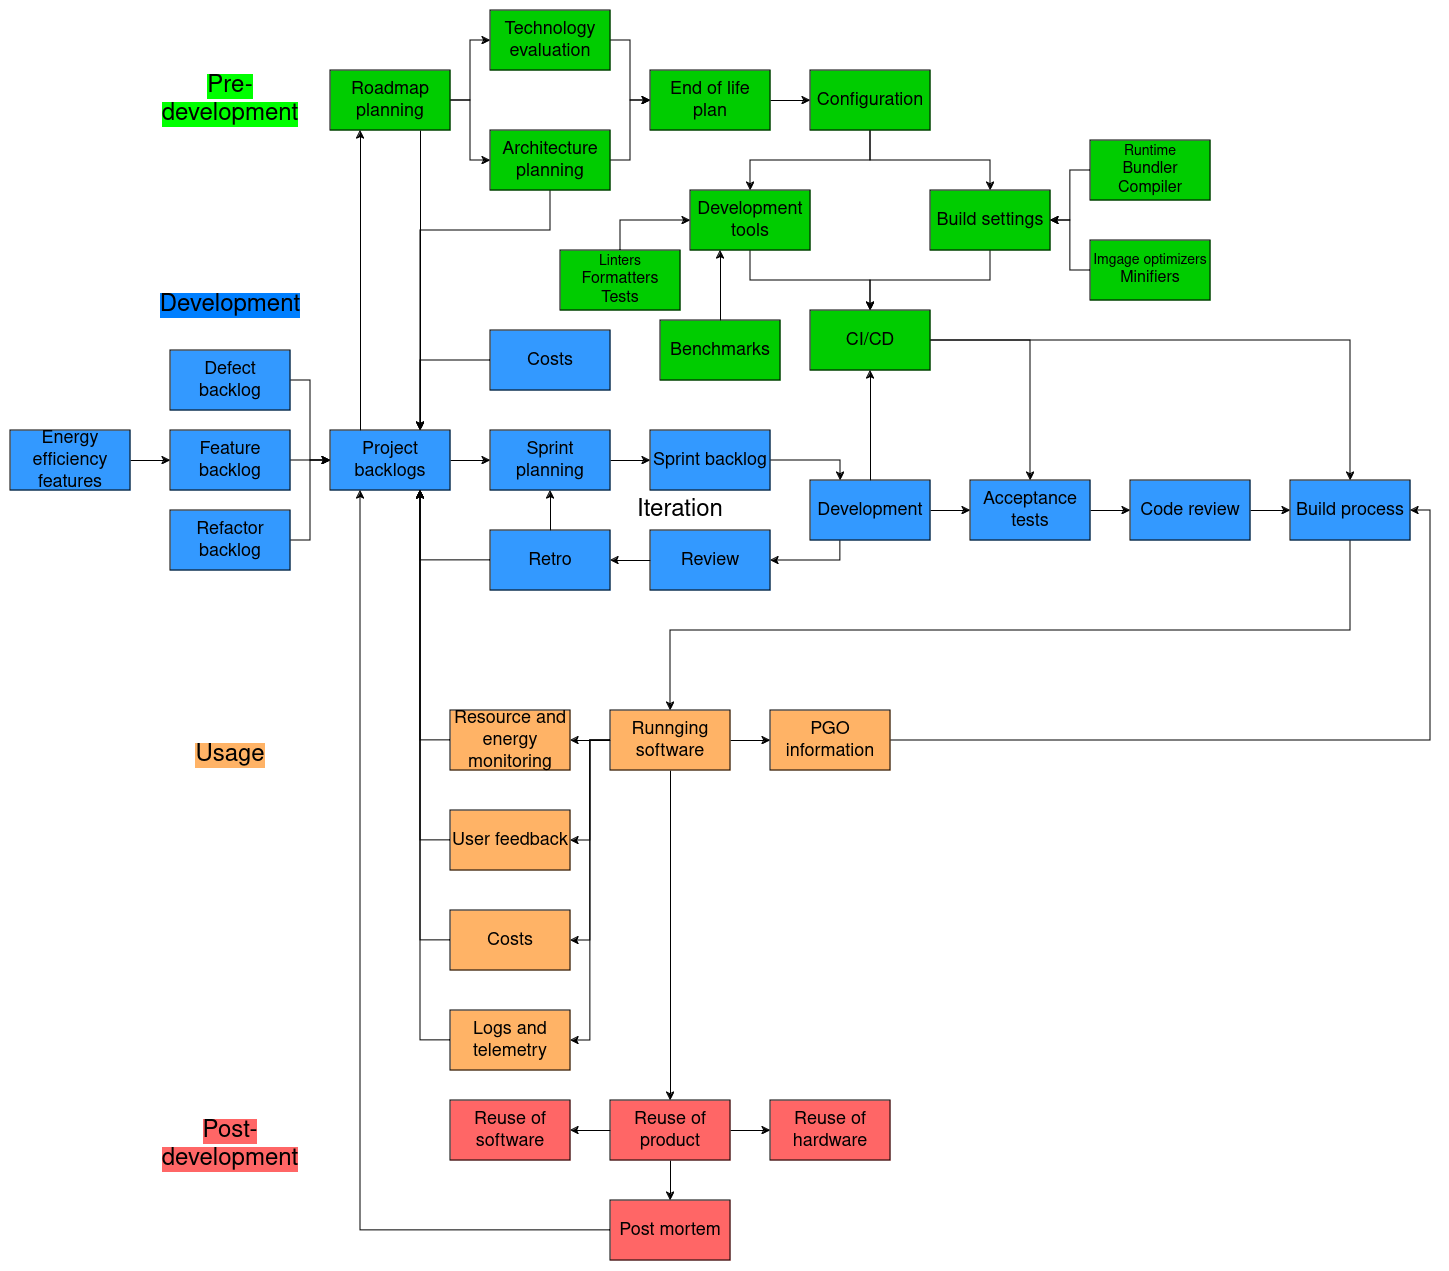
\includegraphics[width=\textwidth]{images/greenagile.png}
\centering
\end{figure}

\subsection{Pre-development Phase}
Many steps can be taken at the beginning of the project that can facilitate a more sustainable development process and end product. These steps often need to be done once per project and sometimes updated during the course of the project but can still have a great impact on the sustainability of the software.

\subsubsection{Roadmapping}
Roadmapping stays mostly the same as in the current model. The core functionality of the product is discussed with the customer and a high-level roadmap is created for the product depending on the feature priorities. These features are then split into epics, which will be further split into user stories. The purpose of this roadmap represent the overall vision for the product and to ensure the project stays true to this vision and does not start adding unnecessary features during development. The roadmap should answer the question of why this software exists. If this question can not be answered, the development should be stopped and the necessity reevaluated as it is the most efficient to not develop anything that is not needed. 

The roadmapping step partially implements the requirements engineering of the Green model for sustainable software engineering shown in Section~\ref{greenmodelforsustainable} by helping determine if the software should be built to solve the problem of the customer. It also creates an outline of the services and features as a roadmap. Risk analysis in terms of energy usage is left out as there is no way to accurately estimate energy usage this early in the project. Requirements testing is also left out as the requirements presented here are meant to indicate what the product needs to do on a high level, meaning they can well be changed during the development.

\subsubsection{Architectural Planning}
The architecture of the software should be planned so that it is extensible enough that features can be easily added but are not too complex. The architecture plan should account for the architecture of the whole software stack including frontend, backend, databases, and hosting platform as well as the architectures of these parts individually. The result of this should be a document describing the high-level architecture of the software stack as well as the high-level architectures of the individual parts of the stack.

Section~\ref{architecture} introduced the following considerations for the architecture of software from a sustainability perspective: \textbf{Caching} and \textbf{bulk requests}, \textbf{data structures and algorithms}, \textbf{error handling}, \textbf{logging}, \textbf{offloading}, and \textbf{indexing}. Many choices made during architectural planning are likely to reappear in day-to-day development work and should follow the same principles as outlined in this step.

%Cache and bulk
\textbf{Caching} should be implemented in all levels of software if possible meaning for example that the database should cache indexes and specific query results, backend should cache expensive function results, database query results, and external API results. Frontend should also cache the results of requests to the backend and possible requests to external APIs. Backend and databases should be planned in such a way that clients can fetch all relevant information with as few queries as possible. This can be achieved with good planning and utilizing \textbf{bulk requests}.

% Data structures and algorithms
Some \textbf{data structures and algorithms} can already be decided during the architecture planning of the software. For data structures, these decisions should account for the most common use cases and optimize for access, search, insertion, or deletion speed based on the use cases. The same applies to algorithms. Decisions on what algorithms are used should take the use case into account and in cases such as password hashing algorithms, find a balance between security and required computation. For both data structures and algorithms optimizing for speed is more important than optimizing for memory.

% Error handling
Architecture should also include details such as how \textbf{errors are handled}. While error handling is largely dependent on the chosen languages and error handling paradigms used by them, there should be some outline of how the errors are propagated through the software and gracefully handled to prevent unexpected errors from crashing the software. 

% Logs
In addition, the architecture should outline what should be \textbf{logged} in the software to catch helpful information about errors and usage. Good logs are vital for finding issues with the software but not everything should be logged as outlined in Section~\ref{logs}. At a minimum, any errors and relevant context to their occurrence should be logged. Any additional logs should be carefully reviewed to determine their usefulness.

% Indexing
Architecture should also outline what should be \textbf{indexed} in databases when planning the initial database schemas to ensure the database operates with optimal performance. Any fields that are frequently used to search for items in the database should be indexed.

% Offloading
\textbf{Offloading} specific computationally intensive work to a server can benefit the client application by lowering system requirements and also allow for more centralized caching of computationally intensive calculations. This should also be accounted for in the software architecture.

% Hosting
Infrastructure architecture should take into account the features that will be added according to the roadmap and ensure the chosen infrastructure is scalable for the expected amount of users for the software. Costs are also an important factor as some infrastructure options might be initially sufficient and cheap but become expensive when scaling up. Developer familiarity with platform options is key in predicting these costs and should therefore be a factor when choosing hosting platforms and methods. The choice of service provider should also be affected by how they produce their energy and other factors mentioned in Section~\ref{hosting}. This will not likely have an impact on the energy consumption of the software but it ensures that the energy consumed is produced responsibly. Hosting platforms also provide varying levels of metrics on energy consumption and using the platform with the most accurate tools should be considered if possible within other requirements.

This phase implements the design and implementation stages of the green model for sustainable software engineering in Section~\ref{greenmodelforsustainable} by creating a system architecture based on the requirements and guidelines for producing more sustainable software.

\subsubsection{Technology Evaluation}
The technology used for a project often depends on customer requirements such as compatibility and performance and also on potential earlier development work. Section~\ref{technology} outlined different technological decisions affecting the energy consumption of the application. These were \textbf{Programming language}, \textbf{runtime}, \textbf{databases} and \textbf{libraries and frameworks}, and \textbf{large language models}. This step should consider all those decisions.

% Limitations
Platform support can affect what technologies can be used for the project for example not all languages and frameworks are suitable for mobile development or embedded systems. If desired platforms do not have an operating system, using low-level languages such as C or Rust is often required.

% Languages
Faster \textbf{programming languages} allow using less powerful hardware to serve the same amount of users as less performant languages with more powerful hardware which also saves in hosting and usage costs making it more sustainable both economically and environmentally. Performance is also especially important on serverless functions platforms as they are often billed by usage time. On serverless platforms, the startup time of the software is crucial for ensuring users do not need to wait too long when using an application. Using performant technologies also allows for higher scaling for lower prices.

% Runtimes
Even if the language used is not the most efficient such as many interpreted languages, the choice of \textbf{runtime} can significantly improve the performance and by extension energy consumption. For example, JavaScript developers should consider Bun as runtime instead of Node due to it being more efficient as mentioned in Section~\ref{runtime} while not being that different from using NodeJs in practice.

% Error handling
Another consideration is how a language or framework handles errors. Making as many errors recoverable as possible is usually better than crashing and restarting the application. To this end technologies that use errors as values and are null safe should be considered provided the team is proficient with them as they can help developers make sure all errors are handled and reduce the rate of unexpected crashes. These kinds of technologies can help enhance technical sustainability by making the software more resilient and also easier to refactor as many issues are caught during the build process.

% Dev familiarity
The current development team's expertise in technologies should also be considered. The development team should choose the most efficient technology they are familiar with and that supports the desired target platforms for the software and configure those technologies to be as efficient as they can. Using familiar technologies allows the team to make better quality software making it more technically sustainable.

% Databases
The choice of \textbf{database} often depends on the use case. However, for most cases at least at the beginning of a project a SQL database such as Postgres or MySQL is sufficient and provides good performance and technical maintainability, especially with proper indexing. SQL databases are also well-supported in most cloud platforms and have solid library support in most languages.

% Libraries
\textbf{Libraries and frameworks} should be carefully considered as they can introduce a lot of unnecessary bloat to software. Libraries should accomplish some specific task and the smallest but still actively maintained library should be used. In cases where only some functionality from a large library is needed, it might make sense to only implement the required functionality. Unnecessary libraries were noted to be detrimental in A Green Model for Sustainable Software Engineering in Section~\ref{greenmodelforsustainable}.

In the case of frameworks, first, it should be evaluated if a framework is even needed. If it is, the choice should be based on performance and available features, not just on what the development team has previously used. Unlike new languages, the time required to learn framework-specific features is often much shorter if the language used in the framework is familiar to the developers.

% LLMS
As mentioned in Section~\ref{llm}, some technologies such as \textbf{large language models} can consume large amounts of energy and there are considerations when using them. For LLMs, the smallest model that fits the requirements should be used. The usage of these technologies should also be carefully considered as more traditional approaches can often be sufficient.

\subsubsection{End of Life Plan}
Software products should have a plan for when they are eventually deprecated and the data needs to be migrated to different platforms. There should be a plan that includes how to export the data used by the software, what format the data is in, and who can export the data. Open data formats should be used to make the data export and reuse easier. It should also include what will be done with the current software in case of end-of-life. Will it be partially reused, open-sourced, or just thrown away? This plan can change throughout the software lifecycle but thought should be given to this as it will likely affect how development is conducted. For example, if the plan is to eventually open source the project, special attention needs to be paid to not use any proprietary code or other media that cannot be open-sourced. Open sourcing specifically should be considered as even if current users might eventually not need the software, someone else can benefit from it and it might even lead to them not needing to develop another comparable product themselves.

\subsubsection{Configuration}
Depending on the technologies used, different configuration options can be used to drastically improve the performance and resource usage of the application as mentioned in Section~\ref{configuration}. Out of the box, many languages have a separate development mode for fast builds and iterations and a production mode for faster runtime performance and smaller bundle sizes. However, these configurations can often be further improved for specific situations and developers should not rely on default options being the best for their use case. During the configuration step, the target platform should be taken into account, and configure the software to be as performant on that platform as possible. If the target platform is a browser or embedded device, it might make sense to optimize for size to ensure minimal network traffic or to ensure that the program can fit the device.

\subsubsection{Development Tools}
Different development tools such as linters and formatters should be used to improve overall code quality and consistent formatting of the code. Running these tools locally also reduces unnecessary CI/CD runs as the code is already compliant with formatting and linting settings enforced in CI/CD pipelines.

Developers can also use tools to assist in writing more efficient software. These tools should present minimal overhead for the developer. This is often achieved by integrating these tools directly with the editors. Static code analyzers are great for integrating with build pipelines as well as the developer's development environment. While tools for directly finding energy patterns in code are still lacking, tools for writing more performant code exist. Depending on the technology used, there are tools such as SonarLint~\cite{sonarsourceLinterTool} that can give hints on writing more performant software. These kinds of tools should be known and recommended in projects by the lead developer depending on the technologies used. They should also be included in the CI/CD pipelines to enforce compliance with them.

Tests should be used to help maintain code quality by detecting issues as early as possible. There are many types of tests such as unit tests, integration tests, end-to-end tests, and testing methods such as property-based testing and fuzzing. Relevant testing approaches are determined by the nature of the project and should be chosen so that they help in detecting issues in the software but do not cause unnecessary overhead to developers.

Benchmarks can be used to catch regressions in the performance of the application or enforce limits on certain features based on what is acceptable according to customer needs or the definition of done. Performance correlates strongly with energy consumption and therefore this can be useful in estimating changes in energy consumption of a specific part of the software. Benchmarks, like tests, can be used as part of the definition to prevent new features and changes from raising the execution time of some features more than is acceptable. They can also be included in CI/CD pipelines to follow changes in performance and energy consumption~\cite{twinsorfalseffriends}.

\subsubsection{Build Settings}
\gls{pgo} is a technique that can be used to improve performance in some compiled languages by compiling software with it enabled, collecting produced data from the production environment, and feeding it back to the compiler during the build step. This allows the compiler to make use case-specific optimizations to the software.

% External tools
For many technologies, there are additional tools to make the final product more efficient. Image optimizer tools such as sharp~\cite{pixelplumbingSharpHigh} can be used to automatically convert PNG and JPEG images to newer formats such as AVIF and WEBP during the build process as well as compress images without noticeable quality loss. For web assembly, there are minifier tools such as wasm-opt~\cite{githubGitHubWebAssemblybinaryen} that can be used to reduce the size of the wasm files during the build process. These tools should be set up at the beginning of the project and used in CI/CD pipelines as part of the build process. For JavaScript and Typescript, many bundlers already perform minimization for code and style files. These techniques can be used to make web applications load faster and reduce network traffic.

\subsubsection{CI/CD}
% CI/CD and Development tools
CI/CD pipelines should also be set up at the start of the project to run chosen tools on pull requests. These tools can include testing frameworks, benchmarks, formatters, linters, and other static analyzers. CI/CD pipelines should be configured to use caching for build artifacts and dependencies to keep them from needing to redownload and recompile on every run. Pipelines should also run the fastest tests and tools first and stop running if any tools fail as this prevents running all tools if the result of the combined tests is a failure.

% Unused dependencies
Unused dependencies should be checked as part of testing and release pipelines and removed from the project. Unused dependencies can, depending on the technologies used, slow the software, bloat the bundle size, or increase compile and therefore pipeline execution times. They also cause unneeded network and I/O usage during building as dependencies are downloaded and installed. There are tools for detecting unused dependencies for most major languages. These tools should be integrated into the CI/CD pipeline to check for unused dependencies. Removing unused dependencies is part of reducing the waste defined in Section~\ref{waste} of the software by removing unneeded features from it.

% Dependency vulnerabilities
Automated tools should also be used to catch dependencies that have vulnerabilities so they can be addressed. This is mostly useful for security but also indirectly saves energy as handling issues caused by possible exploitation of these vulnerabilities is sure to consume more energy than patching them preemptively.

% Specialized tools
Tools such as Google's Lighthouse can be run in CI/CD pipelines for web applications to detect performance, accessibility, and SEO issues in front-end applications. The viability of these kinds of specific tools often depends on the nature of the project.

Some tests could also be run only when things relating to them have changed and on some commits, tests could be skipped altogether~\cite{skippedcommits}. For example, all tests should not be run if only some documentation files were updated. Similar to extreme programming presented in Section~\ref{xp}, the build and testing pipeline should take at most 10 minutes. The 10-minute mark can be used as a heuristic that something is wrong with the performance of the pipeline and it should be addressed.

\subsection{Development Phase}
These steps are done once or more times during every iteration, therefore it is important to avoid adding too many things here so as not to distract from the actual development work. Daily scrum was also dropped as a requirement since many teams within Kvanttori have noticed that it does not bring any benefit and serves as an unneeded distraction from actual work as the same effect can be achieved with communication tools used by teams. This observation is likely due to the development team sizes at Kvanttori being often relatively small. Teams may implement this if they feel it is beneficial.

This phase together with the pre-development phase corresponds to the development phase in the Greensoft model's lifecycle of software products in Section~\ref{greensoft}.

\subsubsection{Backlogs}
Backlogs are used to keep track of work that needs to be done. The product backlog keeps track of all the work while the sprint backlog shows work that has been picked for the current sprint. The product backlog is split into feature, defect, and refactor backlogs. Kanban board presented in Section~\ref{kanbanmethod} can be used to implement these backlogs, as many Kanban tools allow separating backlog into different sections such as labels or lanes.

% Feature backlog
Feature backlog keeps track of new features that need to be added to the product. These items are often added due to customer or other stakeholder requirements. Items can be also added to enhance the energy efficiency of the software. Such features could be based on the criteria presented in Section~\ref{criteria}. This also partially implements the usage stage of the green model for sustainable software engineering in Section~\ref{greenmodelforsustainable} by implementing features that enhance energy efficiency.

% Refactor backlog
A separate refactor backlog ensures that potential refactors do not get prioritized as is often the case if they share the backlog with features. Developers should keep an eye out for potential refactoring opportunities and streamlining of functionality on features done earlier in the project to ensure the project does not become too complex and accumulate technical debt. There is research suggesting that some refactors can improve the energy efficiency of software~\cite{refactorforenergyefficiency}. There seems to be a problem where the need for refactors is recognized during the project but no time is given to do them as they do not seem to immediately give value to the customer. These slowly accumulate technical sustainability debt and make adding new features harder to do correctly without workarounds~\cite{sustainabilitydebt}. Any potential refactors should be reported to the product owner who will then add them to the refactor backlog. If there are items in the refactor backlog, at least 10\% of the sprint effort must be spent on those items to ensure that architectural, technical, and sustainability debt cannot accumulate in the software. In addition to developer feedback, adding items to the refactor backlog is informed by customer feedback and energy and resource usage reported by the hosting environment of the application in addition to error logs and telemetry data collected from the hosting environment.

% Defect backlog
A separate backlog for defects in software should also be set up. This is important to keep track of the \gls{technicalsustainability} of the project and ensure defects cannot accumulate in software. As with refactor backlog, at least 10\% of sprint effort should be spent on fixing defects and as with refactor backlog, the percentage will likely change during the project depending on the speed defects are accumulating.

\subsubsection{Development and Energy Efficient Choices}
% UI design
Section~\ref{methods} outlined methods for ensuring UI design facilitates more efficient software. The UI/UX design should try to minimize the amount of actions required from the user to perform some task within the software. Dark colors should be preferred for better energy efficiency with OLED displays. Visual elements such as animations should also be used sparingly.

Accessibility also needs to be taken into account to improve the software's energy efficiency. If the software does not support accessibility tools such as screen readers, the likelihood of misinputs by users relying on those tools increases which in turn increases the energy usage of the application. The minimum requirement for front-end applications should be the Google lighthouse accessibility check.

% Data structures and algorithms
There will likely be many times during the development when developers need to choose data structures and algorithms to solve a specific problem or to add some feature. These decisions should use the same criteria as the architecture planning step. That is, choose the algorithms based on the use case, prefer lower time complexity over lower space complexity, and find a balance between usability and robustness. The same applies to other part of the architecture planning. Adding new indexes to the database, creating features that make requests to the database or external services, or adding error handling to new features should follow the patterns outlined in the architecture planning step and enforced by the lead developer during code reviews.

This step partially implements the usage stage of the green model for sustainable software engineering in Section~\ref{greenmodelforsustainable} by making software as simple as possible to allow users to perform as few actions as possible to achieve a specific task with the software.

\subsubsection{Acceptance tests}
Tests and other development tools such as formatters and linters that have been set up during the pre-development phase and those added later during the development should be automatically run on code pull requests to enforce code quality.

This step implements the testing stage of the green model for sustainable software engineering in Section~\ref{greenmodelforsustainable} by discovering defects in software before taking it to production. This also partially implements the analysis stage as benchmarks are run during this step.

\subsubsection{Code review}
During code review the lead developer should review the code and ensure it follows the architecture created during the architecture planning and also make sure the code follows sustainable software principles such as using caching, correct data structures and algorithms, and handling error cases properly.

\subsubsection{Review}
In addition to the current model's review step, stakeholders should be made aware of the different measurements collected during the projects such as costs, energy and resource usage, and \gls{technicalsustainability} metrics.

\subsubsection{Retro}
Similarly to the review, the retro step stays mostly the same in the new model. This step should be used to collect developer feedback for the refactor and defect backlogs. It should also be used to discuss the usefulness of the different phases and tools and their effects during the sprint.

\subsection{Usage Phase}
This phase will likely have a lot of overlap with the development phase as the software will be used by the customers during the development in an ideal setting. During the usage phase, the software should be monitored for errors and warnings. Resource usage and energy consumption should also be monitored in addition to costs of usage including those from possible third-party APIs and the hosting platform. These metrics can inform the product owner on what to prioritize in the refactor backlog and feature backlog. Resource usage metrics can also reveal opportunities to downscale hardware needed to run software which in turn reduces running costs. In addition, users should have a channel to provide feedback to the product owner who can relay it to the development team.

This phase implements the rest of the analysis and usage stages of the green model for sustainable software engineering mentioned in Section~\ref{greenmodelforsustainable} by collecting energy usage and resource utilization metrics as well as feedback from the usage environment to inform further development. This phase together with the development phase also corresponds to the usage phase in the Greensoft model's lifecycle of software products in Section~\ref{greensoft}.

\subsection{Post-development Phase}
This phase starts after the active development is either complete or finished for some other reason. This can be because the project moves into maintenance mode or the development is stopped but the software remains in use. This can also happen when the software is deprecated and is ready for disposal.

\subsubsection{Reuse}
After the project is done, there should be a session where internal tools developed to help build the product and functionality written for the product are analyzed for possibilities of reuse in the next projects. In addition, possible hardware such as development kits should be repurposed. This can mean moving internal tools to separate repositories, separating some functionality to separate library packages, and reusing the same hardware kits in future projects. This can help save time and energy in the next projects. The tools and libraries produced from this step should be open-sourced if possible so others will not need to develop the same functionality again later. 

This step implements the recommendation from the Green model for sustainable software engineering in Section~\ref{greenmodelforsustainable} for recycling hardware and software during disposal with the difference that this step can be conducted during development for example in case of software being moved to maintenance.

\subsubsection{Disposal}
The disposal step is used only if the software comes to the end of its lifecycle during the project. This step implements the disposal stage of the Green model for sustainable software engineering in Section~\ref{greenmodelforsustainable} and the end-of-life phase in the Greensoft model's lifecycle of software products mentioned in Section~\ref{greensoft}.

During this step, the end-of-life plan is used to migrate all needed data to a new platform, destroy or archive unneeded data depending on the requirements, and archive, destroy, or open-source the old software. The initial end-of-life plan should be reevaluated for the last time here as some things may have changed since it was last been updated.

\subsubsection{Post mortem}
Post-mortem stays mostly the same as in the current model. The project is reviewed as a whole and learnings are written down to be used in future projects. In addition to this, all the metrics collected during the project should be used to support the review to see what worked and what did not.

\subsection{Metrics}
The phases must produce concrete measurements and other documentation to allow for following the energy consumption of the application and making decisions based on that. The model should implement metrics mentioned in Section~\ref{susmetrics}.

\subsubsection{Energy Consumption and Resource Usage Measurements}
Users should have constant access to the test environment for the software being developed. This environment should have some monitoring software running that produces reports of the energy consumption on set intervals, for example, every sprint. This report can be used when determining the sprint backlog for the next sprint. This kind of reporting should also be done in the production environment for the application to gather data from actual use cases of the software. Out of the different tools presented in Section~\ref{tools}. Many of the tools are easy to integrate into any running server-side web application. Schapandre~\cite{scaphandre} for example can be run with a single docker-compose command and the dashboard provided via Grafana can be customized to show the most important processes and their energy consumption. These tools can be used to implement both the sustainability reporting and the monitoring ability mentioned in the administrative process in the Greensoft model in Section~\ref{greensoft}.

\subsubsection{Costs}
Costs should be monitored and actions should be taken to reduce them when possible. Most hosting and cloud service providers allow monitoring and sometimes even limiting costs easily. In case of costs rising unexpectedly, item should be added to refactor the backlog to solve or mitigate the issue. The cost measurement steps, that being development cost and usage costs implement the lifecycle cost indicators of the Green model for sustainable software engineering in Section~\ref{greenmodelforsustainable}.

\subsubsection{Story points in backlogs}
Story points in different backlogs used in the model are tracked to determine the \gls{technicalsustainability} of the software. Too much work, meaning too many story points, in defect or refactor backlogs can indicate problems with technical debt or insufficient quality control. Story points also allow monitoring of the velocity of the development team.

\subsubsection{Unhandled errors}
Error logs collected from the usage environment can reveal unhandled error cases which can indicate poor technical sustainability and issues with the current software architecture.

\subsection{Roles}
Overall no new roles need to be added to the current process but all existing roles, those being: Product owner, Scrum master, lead developer, and development team, should have at least a basic understanding of green software principles. With some roles requiring a deeper understanding of the subject. Organizations likely need to adopt a learning plan to ensure all members of the development teams have the required skills.

\subsubsection{Product owner}
In addition to product owner duties in the old model, product owners should have knowledge of the sustainability features so they can be added to backlogs and prioritized properly. Additionally, the product owner will be responsible for following the reports from the hosting environments and determining if changes in energy consumption warrant further investigation and potential additions to the refactor backlog.

\subsubsection{Lead developer}
Lead developers are often the senior developers at an organization and should have substantial knowledge of sustainable software development practices. They are responsible for the technology choices, architecture planning, and configuration and should therefore also have knowledge of sustainable architecture patterns and different technologies and tools and also be familiar with their sustainability characteristics such as energy usage and costs. They should be able to recognize the common sources of energy consumption in software, and how to minimize the impact of those.

\subsubsection{Scrum master}
The role of a scrum master stays the same as a facilitator of the development process. Scrum masters should be familiar with the different phases and steps of the proposed model and ensure they are done properly.

\subsubsection{Developer}
All developers should have at least a basic understanding of green software principles and how to make decisions that facilitate the efficiency of the software in day-to-day programming work. For example how to implement a caching system for a specific component. Developers should also be able to configure their development environment with tools recommended by the lead developer.

\subsubsection{Stakeholder}
In addition to the old model, stakeholders should be made aware of the different metrics by not just offering access to them but going over them in reviews. This increases stakeholder awareness of the sustainability effects of the software.

\section{What changes were made to current agile implementation}
Figure~\ref{dev} illustrates what was added to the current model. Existing parts of the model were also modified to include steps facilitating sustainability. The goal of these changes was to fit into the existing model and be light enough that they do not take too much time away from the actual development work while also helping in developing more sustainable software. The model should also as a reference for starting a new project when setting up the development and building environments.

\begin{figure}[H]
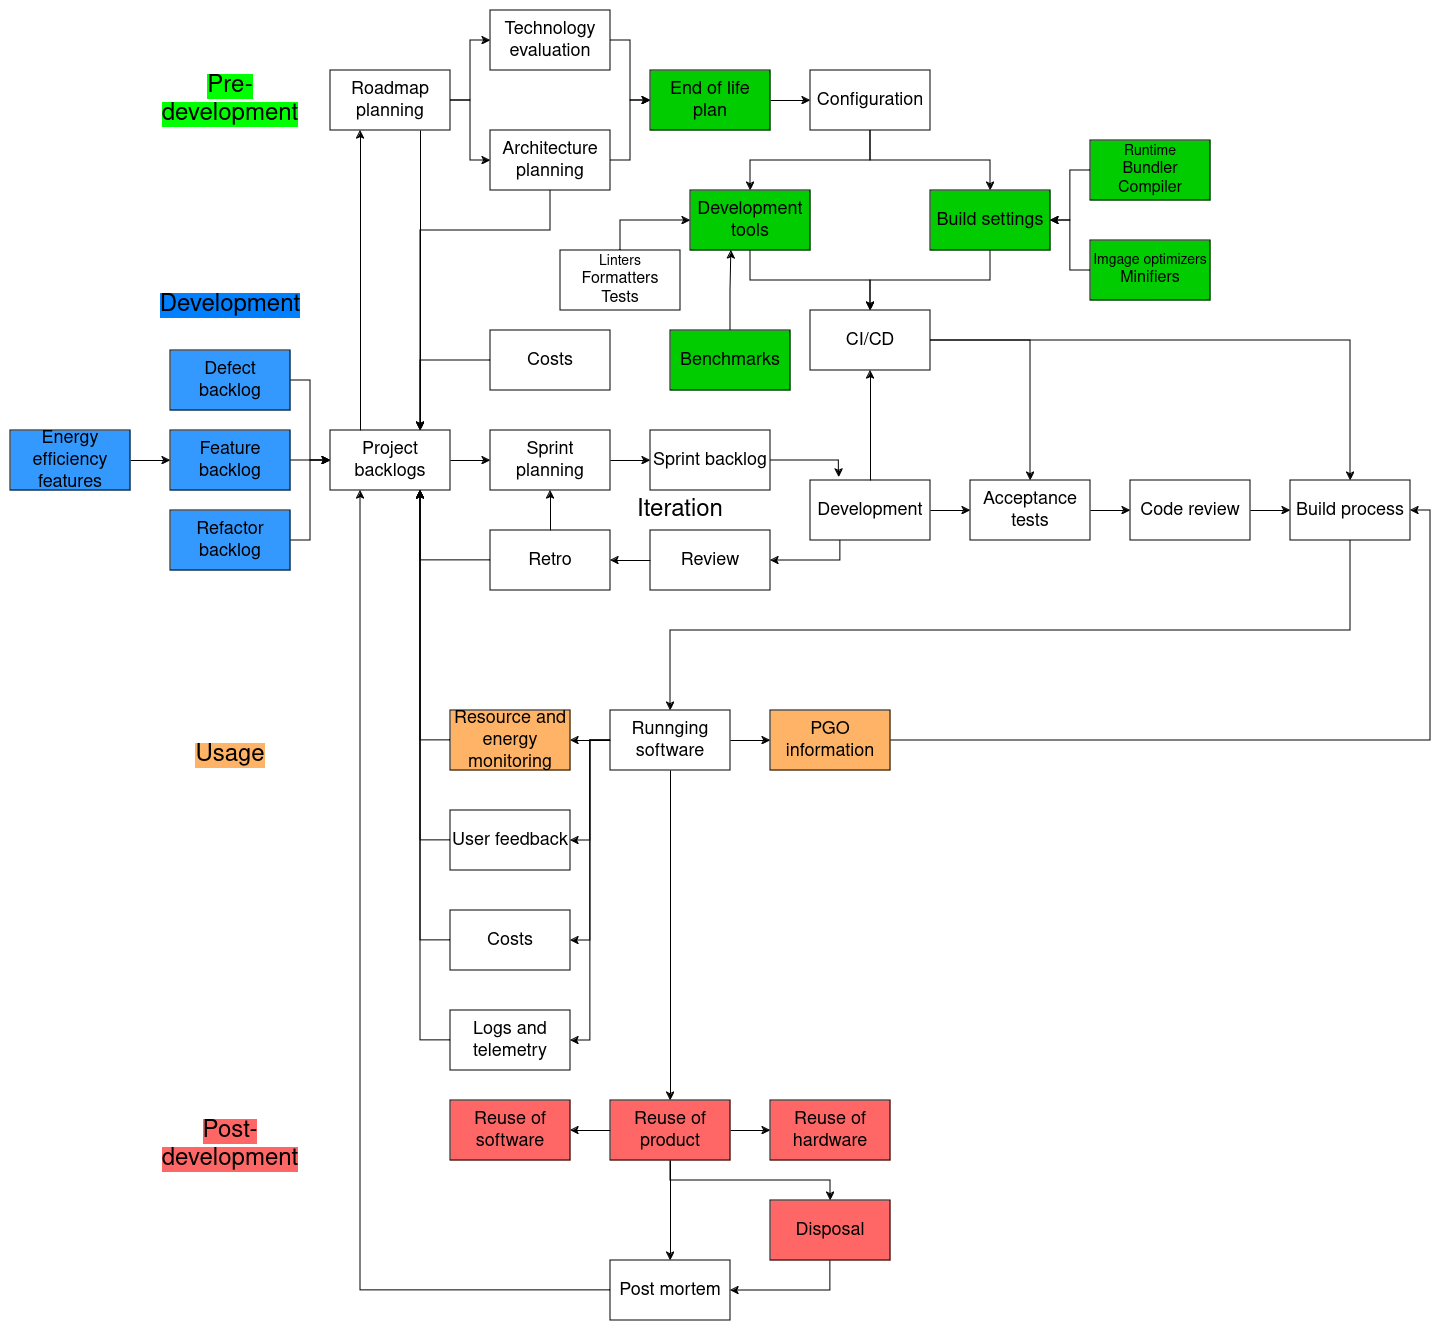
\includegraphics[width=\textwidth]{images/highlighted.png}
\centering
\caption{Highlighted additions of the proposed model}
\label{dev}
\end{figure}
\chapter{Validating the framework}\label{chapter6}
This chapter explains how the proposed model is validated. The methods chosen for this thesis are criteria for green agile processes presented in literature and expert interviews. These methods are used to establish the feasibility of the model in an actual software development project.

\section{Research on Evaluating Sustainable Software Development}\label{criteriaeval}
Existing research on criteria for sustainable software engineering processes was used to extract the criteria from different criteria models and the proposed model was then compared to these criteria to determine how well it fulfills them.

\subsection{Green Agile Maturity Model}
Green Agile Maturity Model by Rashid, Khan, Khan, and Ilyas~\cite{greenagilematurity} lists risk and success factors for green software development processes.  Furthermore, it defines seven green agile maturity levels for the development processes. This model was developed to evaluate software vendors' agile development models from the perspective of sustainable software development.

\subsubsection{Risk Factors}
The risk factors and if they have been mitigated in the proposed model are listed in Figure~\ref{riskfactors}.

\begin{longtable}{ |l|c| }
\hline
\textbf{Risk factors} & \textbf{Mitigated}\\
\hline
Insufficient system documentation & Yes\\
\hline
Limited support for real-time systems and large systems & Yes \\
\hline
Management overhead & Yes\\
\hline
Lack of customer's presence & Yes\\
\hline
Lack of formal communication & Yes\\
\hline
Limited support for reusability & Yes\\
\hline
Insufficient knowledge of the customer & Yes\\
\hline
Lack of long-term planning & Yes\\
\hline
\caption{Risk factors for sustainable software~\cite{greenagilematurity} and if proposed model mitigates them.}
\label{riskfactors}
\end{longtable}

\textbf{The insufficient system documentation} is mitigated by having the roadmap, architectural plan, and end-of-life documents that are kept up to date during the development process.

\textbf{Limited support for real-time systems and large systems} is mitigated as the model does not pose such limitations. In addition, the \gls{technicalsustainability} aspects of the model are helpful when the system's size and complexity increase.

\textbf{Management overhead} is mitigated by using scrum as a basis for the model. The development team is responsible for the project and creating value for the customer.

\textbf{Lack of customer presence} is mitigated by allowing customers access to all information of the development process as well as having them take part in sprint reviews. Customers and the development team also constantly communicate throughout the iteration.

\textbf{Lack of formal communication} is mitigated by available communication tools and stakeholders having to attend at least the sprint review sessions.

\textbf{Limited support for reusability} is mitigated by the reuse step of the post-development phase.

\textbf{Insufficient knowledge of the customer} is mitigated by constant communication as well as the roadmap planning where the customer's business case is presented to the development team and the key features are decided.

\textbf{Lack of long-term planning} is mitigated by the roadmap planning as well as the end-of-life plan done for the project. Additionally, architectural planning takes into account the scaling of the software for future features and users.

\subsubsection{Success factors}
 The success factors and if they appear in the proposed model and if they are included in the proposed model are listed in Figure~\ref{succesfactors}.
\begin{longtable}{ |l|c| }
\hline
\textbf{Success factors} & \textbf{Included}\\
\hline
Accelerated delivery & Yes\\
\hline
Continuous integration & Yes\\
\hline
Continuous validation & Yes\\
\hline
Efficient utilization of time and computing resources & Yes\\
\hline
E-waste minimization & Yes\\
\hline
Flexibility towards change & Yes\\
\hline
Green and sustainable management of product lifecycle & Yes\\
\hline
Improved quality & Yes\\
\hline
Iterative development & Yes\\
\hline
Minimal documentation & Unclear\\
\hline
Minimal reengineering & No\\
\hline
Optimization of processes & Yes\\
\hline
Optimized code & Yes\\
\hline
Polymorphic design & Unclear\\
\hline
Reduced cost & Yes\\
\hline
Rich communication and collaboration & Yes\\
\hline
\caption{Success factors for sustainable software~\cite{greenagilematurity} and if proposed model includes them.}
\label{succesfactors}
\end{longtable}

\textbf{Accelerated delivery} is included in the form of the models underlying scrum processes and delivery following and estimation using the story point system. The model also encourages preventing the accumulation of technical debt that would eventually slow down development speed.

\textbf{Continuous integration} is a core part of the model but the release cycle can depend on what part of its lifecycle software is in and on the teams and stakeholder preferences. Releases can be done once a sprint, multiple times per sprint, or after reaching some feature milestones.

\textbf{Continuous validation} is done via running tests, linters, and other tools to improve the software quality and find issues. Users also have access to the software so it can be tested manually.

The model aims to create more performant software by utilizing many different kinds of tools and architectural patterns so it should have \textbf{efficient utilization of time and computing resources}.

The model \textbf{minimizes e-waste} by producing more performant software allowing the same hardware to be used for more users or in the case of client applications allowing lower-powered hardware to run the application. The hardware reuse step also reduces e-waste by aiming to reuse hardware kits used for development in the future.

\textbf{Flexibility towards change} is included in the form of open communication with stakeholders and iterative development, allowing the features to be added and dropped even on short notice.

\textbf{Lifecycle of the software} is taken into account in different phases of the model.

The model uses automated tools such as linter and tests as well as manual code reviews to maintain and \textbf{improve the quality of the software}.

The model specifies sprints as \textbf{iterations} but does not determine their length as it depends on the project.

The model does not have specifications on \textbf{minimal documentation}. It only requires a roadmap, architectural plan, and end-of-life plan. The model should not produce unnecessary documentation.

\textbf{Minimal reengineering} is not included. The model encourages refactoring to improve efficiency and reduce technical debt.

\textbf{Optimization of processes} is included as every sprint includes a retro where the sprint is assessed by the team and processes that do not contribute value are changed or removed.

\textbf{Polymorphic design} is not included as the model does not specify design patterns that should be used.

Multiple parts of the model aim to \textbf{reduce the costs} of stakeholders both from the development process and running the software.

The model states that stakeholders should be represented in the review sessions, have access to information in all parts of the model, and have a way to constantly \textbf{communicate with the team}.

The model should score well in GAMM~\cite{greenagilematurity} as it includes mitigations for most of the risk factors and includes most of the success factors. 13 out of 16 success factors are included and 8 out of 9 risk factors are mitigated.

\subsection{Assessment criteria for sustainable software engineering processes}
Exploring Assessment Criteria for Sustainable Software Engineering Processes by Wahler, Seyff, and Ramirez~\cite{assesmentcriteriaforsustainable} presents assessment criteria for sustainable software engineering processes. This criteria was developed for a software development industry partner for assessing their development process. The criteria for sustainable software and if they are included in the proposed model are presented in Table~\ref{criteriaforsustainable}.

\begin{longtable}{ |l|c| }
\hline
\textbf{Criteria} & \textbf{Included}\\
\hline
Multidisciplinarity of the Development Team & Yes\\
\hline
Software Engineering Best Practices & Yes\\
\hline
Capacity for Technical Debt Reduction & Yes\\
\hline
Sustainable Collaboration Setup & No \\
\hline
Sustainable Team Culture & No\\
\hline
Ability to Handle Changing Requirements & Yes\\
\hline
Code Maintainability & Yes\\
\hline
Strong Feedback Loops & Yes\\
\hline
Willingness to Change the Process & Yes\\
\hline
Transparency of Communication & Yes \\
\hline
Automatic Quality Checks & Yes\\
\hline
Business Continuity of the Development Environment & Partially\\
\hline
Willingness to Change Requirements & Yes\\
\hline
Implementation of Resource-Intensive Operations & Yes\\
\hline
Sustainable Test Management & Yes\\
\hline
Continuous Sustainability Improvement & Yes\\
\hline
Participation of the Team & Yes\\
\hline
Sustainability in Different Process Phases & Yes\\
\hline
Sustainable Design Decisions & No\\
\hline
Sustainability Reporting & Yes\\
\hline
Implications of Software Operations & Partially\\
\hline
Sustainability Awareness & Partially\\
\hline
Value of Sustainability & No\\
\hline
Availability of Metrics & Yes\\
\hline
Sustainable Procurement and Governance & No\\
\hline
Knowledge about Sustainability & Partially\\
\hline
Development for Efficient Execution & Yes\\
\hline
Sustainability in Release Planning & No\\
\hline
Sustainable Data Structures & Yes\\
\hline
Sustainability Incentive & No\\
\hline
Sustainability Quality Attributes & No\\
\hline
Usage of tools to assess sustainability & Yes\\
\hline
Energy Consumption of the Development Process & No\\
\hline
Different Sustainability Dimensions & Yes\\
\hline
Consideration of Different Orders of Effects & No\\
\hline
Direction and Policies to Improve Sustainability & Yes\\
\hline
Sustainable Infrastructure & Yes\\
\hline
Technologies for System Development & Yes\\
\hline
\caption{Criteria for sustainable software~\cite{assesmentcriteriaforsustainable} and what criteria the proposed model implements }
\label{criteriaforsustainable}
\end{longtable}

\subsubsection{Implemented}
\textbf{The multidisciplinarity of development team} is accounted for in the model as required roles for the development team. \textbf{The engineering best practices} are accounted for mainly in the pre-development phase using development tools and integrating them to CI/CD pipelines which also implements \textbf{Automatic quality checks}. This also allows implementing \textbf{Code maintainability} which is further implemented by enforcing code reviews in addition to automatic checks. The model also enforces allocating development work to defects and refactors from separate backlogs to improve maintainability which also allows for \textbf{Capacity for technical debt reduction}. 

\textbf{The ability to handle changing requirements} is implemented as the process is based on agile principles and works in iterations allowing fast reaction to changes. Similarly, the \textbf{willingness to change requirements} is implemented. \textbf{Strong feedback loop is implemented} by collecting user feedback from the running app and by requiring key stakeholder presence in iteration reviews.

\textbf{Willingness to change the process} is implemented as during the sprint retro the development team will discuss what worked and what did not. These discussions might lead the team to drop some parts of the process model that do not produce any value. In the post-development phase, a larger post-mortem is conducted to inspect the project as a whole and collect findings that can be used in subsequent projects. This might also include adding, dropping, or changing parts of the model to fit the team better.

\textbf{Transparency of communication} is implemented by allowing all relevant stakeholders to access the information about the project. \textbf{Implementation of Resource-Intensive Operations} is included as the model includes many monitoring tools in the usage environment as well as benchmarks to find specific intensive code paths. \textbf{Sustainable Test Management} is implemented as optimizing CI/CD pipelines to run in under 10 minutes and by setting the pipelines up in such a way that tests are not run if not necessary such as with documentation changes.

\textbf{Continuous Sustainability Improvement} is implemented by monitoring usage and running benchmarks to find issues with performance, energy consumption, or resource usage and adding these issues to refactor or defect backlogs so they can be fixed. \textbf{Participation of the Team} is implemented as teams are responsible for implementing the model in their projects in ways that work for them. \textbf{Sustainability in Different Process Phases} is implemented as the model is split into four different phases with each having different methods for increasing sustainability.

\textbf{Sustainability Reporting} is implemented as the model includes many metrics related to different aspects of sustainability, all of which are available to stakeholders. These metrics also allow implementation of \textbf{Availability of Metrics} and \textbf{Usage of tools to assess sustainability}. \textbf{Development for Efficient Execution} is implemented as multiple phases of the model are aimed at optimizing execution efficiency. \textbf{Sustainable Data Structures} is implemented in the architecture planning phase.

\textbf{Different Sustainability Dimensions} are taken into account in the model. \textbf{Technologies for System Development} is implemented as performance and maintainability are considerations in technology evaluation.

\subsubsection{Partially Implemented}
\textbf{The business continuity of the development environment} is partially implemented as the software should be easily changeable based on changing needs. The model also has an end-of-life plan for migrating to new software if necessary. The model however does not use the ability to adapt technologies for new platforms as criteria in technology evaluation. The model considers only the target platforms defined at the start of the project as configuring for those platforms allows for greater efficiency.

\textbf{Sustainability Awareness} is partially implemented as the stakeholders have access to all metrics but they are not required to actively follow them. \textbf{Knowledge about Sustainability} is partially implemented as the development team roles require some knowledge of sustainability practices. This is not required from all stakeholders. \textbf{Direction and Policies to Improve Sustainability} is implemented as the development takes into account regulation and stakeholder needs.

\textbf{Sustainable Infrastructure} is included as the technology evaluation uses the sustainability of infrastructure as a criterion. \textbf{Implications of Software Operations} is partially implemented as the model enforces collecting metrics from different phases but does not require measuring all sustainability aspects in every phase.

\subsubsection{Not implemented}
The model does not take \textbf{sustainable collaboration setup} into account as it does not enforce a specific way of collaborating within the team. Similarly, the model does not say anything about \textbf{sustainable team culture}.

\textbf{Sustainable Design Decisions} is not implemented as the model does not require explicitly documenting the estimated sustainability impact of all design decisions. \textbf{Value of Sustainability}, \textbf{Sustainable Procurement and Governance} and \textbf{Sustainability Incentive} are not included as implementing them is beyond the scope of single development projects.

\textbf{Sustainability in Release Planning} is not implemented as the model makes no specific mention of the release schedule. \textbf{Sustainability Quality Attributes} is not implemented as the requirements are based on stakeholder needs and while the model aims to produce sustainable software, this does not need to be specified in requirements. \textbf{Energy Consumption of the Development Process} is not implemented as there are no tools for reliably measuring the entire development process energy consumption. \textbf{Consideration of Different Orders of Effects} are only partially implemented as the model only accounts for first-order effects.

\subsubsection{Scoring the model}
The model fully fulfills 24 of 39 criteria and 4 out of 39 partially. 3 out of 39 are out of scope for single projects leaving 8 unfulfilled criteria out of 39. This shows there is some room for improvement for the model but implementing all the phases without making the model too heavy to use can be challenging.

\section{Expert interviews}\label{expertinterviews}
The expert interviews were conducted to validate the model against the experiences of developers from different organizations that are interested in green and energy-efficient software.

\subsection{Interview process}
 The model for the interviews is semi-structured. The interview audio was recorded and transcribed with OpenAI whisper model~\cite{whisper} running locally. The transcription was coded and analyzed with QualCoder~\cite{qualcoder}. Coding was then used to quantify feelings towards the model, either positive or negative, and additions or removals from the model.

The following questions are asked during the interview but not necessarily in the same order:

\begin{enumerate}
    \item What is missing from the model if anything?
    \item What would you remove from the model if anything?
    \item Are the metrics proposed in the model effective?
    \item Are the roles in the model useful?
    \item Do you think the model is overall effective in increasing sustainability?
    \item Would you use this model in a project? Why or why not?
\end{enumerate}
    
A thematic analysis was performed for the interviews to find out the effectiveness of the model regarding sustainability, the heaviness of the model, sentiment on the usefulness of the metrics and roles in the model, possible challenges with using the model, and interest in using the model. The interview transcripts were coded with the following codes: Additions / Removal of phases, Negative / Positive on metrics, Negative / Positive on roles, Negative / Positive on usage, Negative / Positive on usefulness, and finally Usage notes to identify what needs to be taken into account when using the model.

Most of the interviews were conducted in Finnish. The quotes from interviews are translated into English and shortened to illustrate the results of the analysis. Original quotes in Finnish are listed in Appendix~\ref{appendixa}.

\subsection{Interview analysis}
The amount of additions was overall high with 3 to 5 additions per interview which might indicate something is missing from the model. Upon further analysis most additions were clarifications and additions to existing phases and are therefore not indicative of the model missing any crucial phases but rather that some parts of the model need further refinement. 

\subsubsection{Additions}
One interviewee noted that \gls{embeddedemissions} is not taken into account in the model. This can affect the overall sustainability as, depending on the platform, \gls{embeddedemissions} can account for almost half of the emissions. This can affect whether the software should be optimized to work on the same devices for as long as possible. \textit{"At some point when newer hardware is more energy efficient, it makes sense to take the \gls{embeddedemissions} hit"}~\hyperref[i14]{[Appendix 1.4]}.

Many interviewees also noted the lack of granular measurements for energy consumption in the model and mapping energy consumption to specific parts of the code. \textit{"Like currently, you can trace single user request through the full stack of the application, you could do the same with the energy used by that single user request"}~\hyperref[i33]{[Appendix 3.3]}. \textit{"So there is currently no tool for following so-called energy hotspots?"}~\hyperref[i43]{[Appendix 4.3]}. This can present challenges due to tooling around granular measurements still being lackluster at best as interviewee 1 noted: \textit{"400 papers about measurements and not one of them was universal in the end"}~\hyperref[i16]{[Appendix 1.6]}.

Two of the interviewees also noted the lack of social and individual sustainability aspects in the metrics. \textit{"There are five of these sustainability aspects and here there are three and the velocity"}~\hyperref[i17]{[Appendix 1.7]}. \textit{"Yes, I don't know, I think that maybe that social aspect. Could something be added to that?"}~\hyperref[i23]{[Appendix 2.3]}.

\subsubsection{Removals}
None of the interviews indicated a desire to remove anything from the model. \textit{"...That I would not remove anything and I don't see anything that would be unnecessary in this."}~\hyperref[i41]{[Appendix 4.1]}. This together with a high amount of positive responses on the usefulness of the model, which there were 2 to 6 per interview, indicates that according to the interviewees, the phases proposed by the model could be effective in increasing the sustainability of the software being developed. There were also no instances of negative comments relating to the usefulness of the model.

\subsubsection{Metrics}
Responses on metrics were inconclusive but more critical as there were 1 to 2 positive comments on metrics and 0 to 5 negative comments on metrics per interview. Negative comments regarding metrics focused on pointing out their simplicity and half of the interviewees desired more complex metrics that combine the proposed metrics, which were useful as the positive comments pointed out, such as measuring the ratio of different backlogs instead of their sizes or combining cost information with sprint velocity or work time. \textit{"So how we can make these into second-level metrics so that there is division and multiplication with something that we can use to compare these between software projects."}~\hyperref[i12]{[Appendix 1.2]}.

\subsubsection{Roles}
Roles were also inconclusive with them mainly being seen as useful and there were some comments regarding the usefulness of some roles such as the scrum master. \textit{"That Scrum master...I'm not necessarily sure why it is needed."}~\hyperref[i34]{[Appendix 3.4]}. The introduction of the tech lead role was seen as positive. \textit{"We have had the tech lead role for a long time"}~\hyperref[i11]{[Appendix 1.1]}. \textit{"As sustainable development is not necessarily a widespread skill, having someone who knows these things can be beneficial"}~\hyperref[i22]{[Appendix 2.2]}. Interviewee 1 noted that organizations could have green coding experts that don't necessarily work full time in the development team but are available for consulting in specific scenarios: \textit{"It could have like a green coding expert that will be used when necessary so that the team does not have to know everything"}~\hyperref[i13]{[Appendix 1.3]}.

\subsubsection{Phases and Steps}
The phases and steps in the model were seen as useful. \textit{"On paper, this should produce more sustainable software if followed completely"}~\hyperref[i24]{[Appendix 2.4]}. Introduction of energy measurement was also seen as especially useful: \textit{"If we can get the energy consumption data, that is something that is not probably used anywhere because there has been no way to get it. That is something new."}~\hyperref[i31]{[Appendix 3.1]}. Architecture and technology evaluation were also seen as useful. \textit{"What was great about it was that every high-level architectural and technology choices guide to the correct direction really well"}~\hyperref[i42]{[Appendix 4.2]}.

\subsubsection{Interest}
All interviewees indicated interest in using the model in software development projects which reinforces the ideas of its overall usefulness. Usage notes highlighted some considerations for taking the model into an actual project, such as the need to adapt it to the processes of the organization implementing it and taking into account the project type. Interviewee 2 noted that the model might not be the best fit for quick prototyping: \textit{"This will be a bit heavier than some regular agile would be...This means that this will have a specific purpose for example if we want high-quality software...But if we make some fast MVPs or other things I, well I don't think that it is the purpose of this, this won't be fit for that."}~\hyperref[i21]{[Appendix 2.1]}. \textit{"I would like to try it. But every model is made for specific context so that won't work for us without some adaptations"}~\hyperref[i14]{[Appendix 1.4]}.

\subsubsection{Conclusion}
Based on the interview analysis the model is seen as useful and mostly includes relevant phases and roles and therefore no new phases or roles need to be added. 

Metrics on the other hand need some revisions to include more complex metrics, however, existing metrics are good and relevant for producing these more complex metrics. These more complex metrics can be produced by measuring ratios of the current metrics. These include development velocity's ratio with development team costs, the ratio between all different backlogs, the ratio of energy consumption with usage costs, and development cost per backlog item among other possible combinations. More relevant metrics are likely to emerge when the model is used in practice. 

Most interviewees indicated the need for fine-grained energy measurement in software but implementing it with currently available tools is not necessarily feasible in this kind of model.

Measuring the social and individual aspects mentioned in two of the interviews is outside the scope of this thesis and becomes more important when measuring the impact of this model on an organizational level.

The green coding expert proposed in the interviews is an organizational role and is therefore outside the scope of this thesis. It does highlight some adjustments that should be made when scaling the model beyond single teams and is a good topic for future research.

There is also a clear interest in using the model in practice to enhance the sustainability of software and its development. Interviewees also noted that there are some adaptations that need to be made to the model before this to adapt it to different company sizes and development processes. This is often the case with all agile processes as no single implementation works for all organizations.
\chapter{Discussion}\label{discussion}
This chapter summarizes the key findings of the thesis, explores their implications for the field of sustainable software engineering, lists potential threats to the validity of this thesis, and lists further research opportunities.

\section{Answers to the research questions}
The research questions of this thesis were:
\begin{itemize}
    \item RQ1: What methods are there for developing sustainable software?
    \item RQ2: How to measure the sustainability of the software?
    \item RQ3: How to integrate sustainable development methods into an agile development process?
\end{itemize}

\subsection{RQ1: What methods are there for developing sustainable software?}
This thesis presents multiple methods for developing more sustainable software in Section~\ref{methods}. Technology choices can affect environmental, technical, and economic sustainability. Configuration can be used to further optimize the sustainability of chosen technologies. Technology choices also affect the technical sustainability of the software as strongly types languages and error handling paradigms where errors are values instead of exceptions allow moving many checks to compile or build time instead of runtime. User interfaces can also have an effect as they affect how many actions users have to do to achieve a specific task with software. UIs also address accessibility concerns as poorly accessible software is difficult to use for users with accessibility tools and causes misinputs which in turn increase energy consumption. Table~\ref{susmethods} lists different methods for increasing the sustainability of software in Section~\ref{methods} and their benefits.

\begin{longtable}{ |p{0.5\textwidth}|p{0.5\textwidth}| }
\hline
\textbf{Method} & \textbf{Benefit}\\
\hline
Use of caching in all layers of software & Improves performance, reduces energy consumption, can reduce hosting costs \\
\hline
Use of bulk requests with network and I/O & Improves performance, reduces energy consumption, can reduce hosting costs \\
\hline
Use of correct algorithms and data structures for the task & Improves performance, reduces energy consumption, improves technical sustainability\\
\hline
Logging only what is necessary such as errors & Reduces energy consumption\\
\hline
Offloading expensive calculations to a server & Reduces hardware requirements of client devices\\
\hline
Indexing database field used for searching rows & Improves performance, reduces energy consumption\\
\hline
Use of high-performance languages & Improves performance, reduces energy consumption, and lowers hardware requirements.\\
\hline
Use of languages with strict, static type systems & Helps catch errors at build time, improves technical sustainability \\
\hline
Use of languages with errors as values and optional types & Helps make sure errors and missing values are handled at build time, improves technical sustainability\\
\hline
Use of faster runtimes in interpreted languages & Improves performance, lowers energy consumption\\
\hline
Use of databases that enforce types such as SQL databases & Improves technical maintainability\\
\hline
Adding only necessary libraries to a project and using small libraries that perform specific tasks & Large libraries can bloat the bundle size of software\\
\hline
Choosing frameworks that are performant and actively maintained. Newer frameworks tend to use newer language features & Improves performance, which can reduce energy consumption\\
\hline
When using LLMs using the smallest model possible for specific tasks & Reduces hardware requirements and energy consumption\\
\hline
Use of smallest data formats that allow representing needed information. For example WEBP or AVIF for images. & Improves performance, reduces costs, improves page load times, lowers bundle sizes\\
\hline
Use of development tools such as linters and formatters & Improve code quality and readability\\
\hline
Running CI/CD pipelines only when necessary & Reduces energy consumption and costs\\
\hline
Preferring hosting services using clean energy & Reduces carbon emissions\\
\hline
Configuring technologies used for target platform & Improves performance, reduces energy consumption\\
\hline
Designing UIs to be as simple as possible & Reduces energy consumption, improves user experience\\
\hline
Making software accessible & Reduces energy consumption by preventing misinputs, improves user experience\\
\hline
Use of dark colors & Reduces energy consumption on OLED devices\\
\hline
Allowing users to disable unneeded features & Reduces energy consumption\\
\hline
Showing users energy and resource usage & Can lead to reduced energy consumption\\
\hline
\caption{Methods for increasing sustainability of software in Section~\ref{methods}}
\label{susmethods}
\end{longtable}

\subsection{RQ2: How to measure the sustainability of the software?}
Chapter~\ref{chapter4} presented metrics and measurement tools for different sustainability aspects. Many monitoring tools are available especially for web applications that allow measuring the environmental sustainability by measuring energy usage of the software. Economic sustainability can be measured by monitoring the costs of hosting platforms, version control services, and other development tools in addition to the costs of the development team. Technical sustainability can be measured by using project management tools that allow labeling user stories as features, defects, and refactors and measuring the number of story points assigned to each category. Story points can also be used to measure development velocity. Sustainability metrics presented in Section~\ref{susmetrics} are listed in Table~\ref{measurements}. These metrics can be further combined to measure ratios between different metrics.

\begin{longtable}{ |p{0.5\textwidth}|p{0.5\textwidth}| }
\hline
\textbf{Measurement} & \textbf{Sustainability aspect}\\
\hline
Amount of work in features & Technical\\
\hline
Amount of work in defects & Technical\\
\hline
Amount of work in refactors & Technical\\
\hline
Error logs from unhandled errors & Technical\\
\hline
Development velocity of the team & Technical\\
\hline
Cost of development team & Economic\\
\hline
Cost of development tools & Economic\\
\hline
Cost of hosting & Economic\\
\hline
Energy consumption of software & Environmental\\
\hline
Energy consumption of infrastructure & Environmental\\
\hline
Resource usage of software & Environmental\\
\hline
Performance benchmarks of software & Environmental\\
\hline
\caption{Sustainability metrics presented in Section~\ref{susmetrics}}
\label{measurements}
\end{longtable}

\subsection{RQ3: How to integrate sustainable development methods into an agile development process?}
This thesis presented a sustainable agile development model that integrates sustainable software development practices into the agile process used by Kvanttori. This model was presented in Section~\ref{susimplementation} and further validated in Chapter~\ref{chapter6}. Integrating these practices was done by implementing parts of the models proposed in earlier research on sustainable software development processes in Chapter~\ref{chapter3}, using methods from research on what affects sustainability in Section~\ref{methods} to add concrete steps for increasing the sustainability of the software and its development to different phases of the model and adding metrics and tools for different sustainability aspects in Chapter~\ref{chapter4}. The model was validated with existing criteria on sustainable agile processes in Section~\ref{criteriaeval} and mostly fulfilled the relevant criteria within the scope of the model. Expert interview validation in Section~\ref{expertinterviews} also reinforced the usefulness of the model and interest in using it. The final model in Section~\ref{susimplementation} is pictured in Figure~\ref{final}.

\begin{figure}[H]
\caption{Final model including metrics and roles in Section~\ref{susimplementation}}
\label{final}
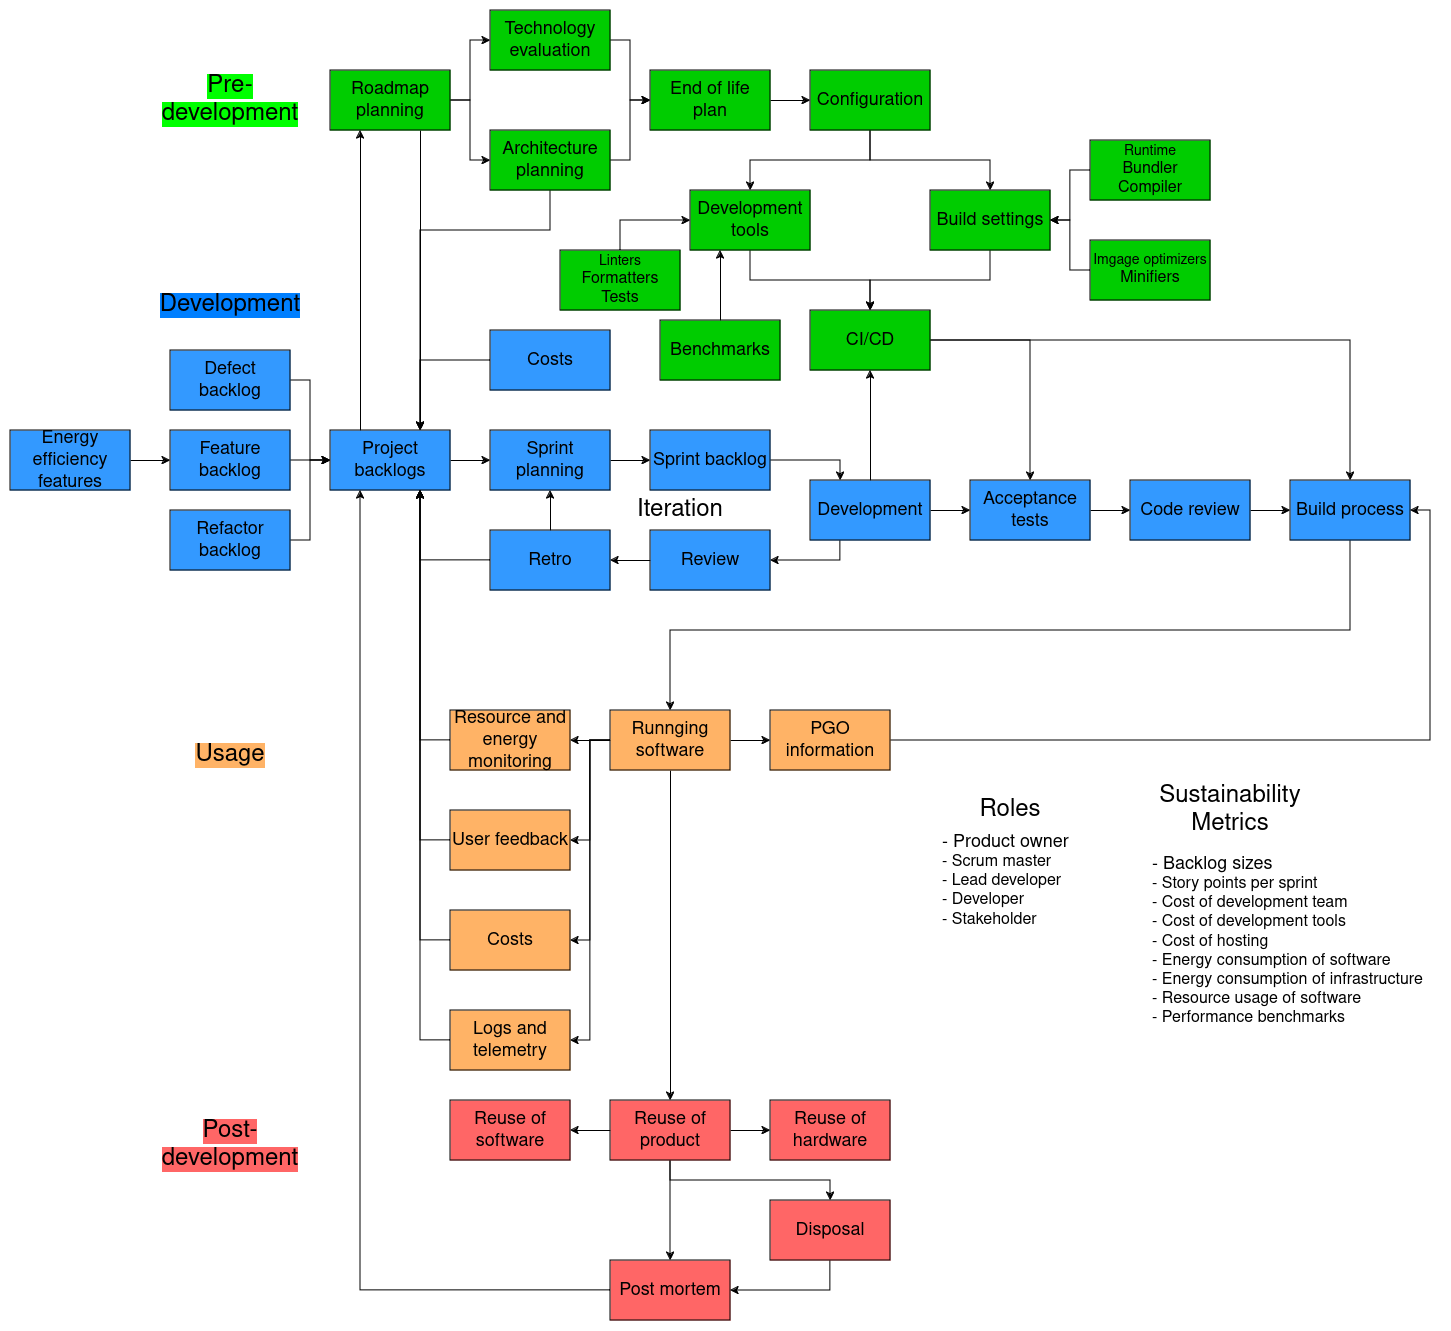
\includegraphics[width=\textwidth]{images/result_model.png}
\centering
\end{figure}

The results of the validation with sustainable software development process criteria in Section~\ref{criteriaeval} are presented in Table~\ref{scores}.

\begin{longtable}{ |p{0.5\textwidth}|p{0.5\textwidth}| }
\hline
\textbf{Measurement} & \textbf{Score}\\
\hline
Green agile maturity model risk factors & 8/8 mitigated\\
\hline
Green agile maturity model success factors & 13/16 included\\
\hline
Assessment criteria for sustainable software engineering processes & 24/39 fulfilled\\
\hline
\caption{Scoring of the model using existing green agile criteria in Section~\ref{criteriaeval}}
\label{scores}
\end{longtable}

The results of the interview validation in Section~\ref{expertinterviews} are presented in Table~\ref{interviews}.

\begin{longtable}{ |l|c|c|c| }
\hline
\textbf{Times themes appeared in interviews} & \textbf{Avg} & \textbf{Mod} & \textbf{Dist}\\
\hline
Additions & 4,5 & 5 & 5, 3, 5, 5\\
\hline
Removals & 0 & 0 & 0, 0, 0, 0 \\
\hline
Positive on metrics & 1.5 & 1.5 & 1, 1, 2, 2\\
\hline
Negative on metrics & 2.5 & 2.5 & 0, 2, 3, 5\\
\hline
Positive on Roles & 0.75 & 1 & 0, 1, 1, 1\\
\hline
Negative on Roles & 0.75 & 0.5 & 0, 0, 1, 2\\
\hline
Positive on Usefulness & 3.5 & 3 & 2, 2, 4, 6\\
\hline
Negative on usefulness & 0 & 0 & 0, 0, 0, 0\\
\hline
Positive on usage & 1.25 & 1 & 1, 1, 1, 2\\
\hline
Negative on usage & 0 & 0 & 0, 0, 0, 0\\
\hline
Usage notes & 3.5 & 4.5 & 0, 4, 5, 5\\
\hline
\caption{Average, median, and distribution of comments for each code per interview in Section~\ref{expertinterviews}}
\label{interviews}
\end{longtable}

\section{Implications}
This thesis was able to create a concrete implementation of existing sustainable software practices and agile processes by implementing phases of existing sustainable software development processes and combining them with researched methods of increasing software sustainability across different sustainability aspects. This shows that it is possible to make use of these models in software development to potentially improve sustainability. This should be used as a starting point to adapt more theoretical sustainable development processes and methods into use in software development companies. Companies should start adapting these kinds of models into their development processes to test their effectiveness and to improve the sustainability of their software.

\section{Threats to validity}
The validation using the existing research on sustainable software criteria might have been affected by the author's bias as the creator of the model which might have caused the evaluation of the model to be more positive, especially in cases where the description of some criteria was unclear.

All interviewees were interested in sustainable software development and had some previous knowledge of what methods can be used to make software more sustainable. This might have led them to view the model in a more positive light as opposed to someone who is skeptical of the benefits of sustainable software development. 

The interviewees did not necessarily take the same amount of time to familiarize themselves with the model before the interview which might cause some differences in the answers as they are dependent on the understanding of the model as some interviewees might have had a better understanding of the proposed model beforehand.

The amount of interviews in the interview part of this thesis was low which might have caused these interviews to not be representative of the opinions of the majority of software engineers or experts in sustainable software.

The model has not been used in an actual software development project as this thesis did not include a case study of the model. This is important as real-world scenarios can reveal unexpected challenges in software development processes.

\section{Further Research}
One of the main limitations of measuring the energy consumption of software is measuring the energy consumption of single functions and methods. A tool that allows writing unit tests for energy consumption would make following and improving the energy consumption of specific functionality much easier. While some tools do exist, no easily available and actively maintained testing framework exists for energy consumption.

Another potential avenue of research would be actual case studies from projects using this model to find out how the sustainability aspects would be affected. Such case studies would help determine what parts of the model are effective and what parts are difficult to implement in real-world scenarios.

Further research could be conducted on what changes need to be made to adapt the model for scaling scrum frameworks such as Safe, Less, or Scrum at scale. This could also take into account what can be added to the model on an organizational level. This could include what roles the organization needs in addition to those in the project teams, how organizations can track the evolution of sustainability in their projects, and how organizations can minimize e-waste for example by preferring refurbished computers. Organizations could also include the social and individual sustainability aspects and metrics for measuring them to the model.

The proposed model focuses primarily on web applications. Further research should be conducted on how the model can be optimized when focusing on specific software domains such as native applications, mobile, or embedded systems.
\chapter{Conclusion}\label{conclusion}
This thesis presented a literature review to find out what affects the sustainability of the software, how current agile methods account for sustainability, and how to measure the sustainability of the software. A new model for developing more sustainable software was created based on the current model used at a software development company called Kvanttori by adding relevant methods and metrics from the literature review. This model was then validated with existing criteria for sustainable development processes found in literature and expert interviews from developers at Kvanttori as well as external experts on sustainable software.

The literature review identified multiple relevant methods for increasing the sustainability of the software including the choices of architectural patterns, technologies, and hosting platforms. The literature review also found existing agile models for sustainable software which included sustainability-enhancing steps such as disposal of software, requirements engineering, and measuring energy consumption. Finally literature review identified multiple metrics and measurement tools for measuring different aspects of sustainability including easy-to-set-up tools for server environments for measuring the energy usage of different software applications running on the server. These findings combined with the existing methods used at Kvanttori produced a model that accounts for sustainability in different parts of the software development project and based on the expert interviews, should allow for making more sustainable software.

The model presented in this thesis can be used by software development companies to better implement methods to increase the sustainability of software in their development processes. The model can also be further specialized depending on the domain of software development it is used in such as embedded systems, mobile or native applications. Some additions need to be made when moving the model from a project level to an organizational level such as taking the larger sustainability impact including the social and individual aspects into account.
% The thesis main content ends here.
\printbibliography
\appendix

\chapter{Original quotes in Finnish}\label{appendixa}

\section{Interviewee 1}
\subsection{}\label{i11}
"Meillä on toi, Tech leadina, toi Lead developer rooli ollu pitkää."
\subsection{}\label{i12}
"Että mitenkä näistä saa niinkun toisen tason mittareita. Että niitä niinkun. Tulee jakolaskua tai kertolaskua jonkun jutun kanssa, jolla voidaan sitten ruveta saamaan jotain vertailtavuutta niinkun eri softien yli."
\subsection{}\label{i13}
"Sillä vois olla sellanen niinku Green code expert, jota käytetään silloin kun on tarve, että vältetään se, että kaiken tiedon ei tarvi olla siinä tiimissä."
\subsection{}\label{i14}
"Kyllä mä haluaisin kokeilla. Siis se, että jokainen mallihan tehdään niinku kontekstiin. Niin toi ei ihan suoraan meille uppoa."
\subsection{}\label{i15}
"Että jossain kohtaa, kun uudempi rauta on modernempi rauta, energiatehokkaampaa,
milloin kannattaa ottaa se Embedded Emissions-isku ja vaihtaa se rauta sieltä alta."
\subsection{}\label{i16}
"Pintapuolisesti mittauksesta löytyi 400 paperia, tai muutaman vuoden vanha kirjallisuustyö, missä oli 400 paperia mittaamiseen liittyen ja yksikään niistä ei loppupelissä ollut sellainen universaali."
\subsection{}\label{i17}
"Tässä nyt on viisi oli niitä sustainability kulmia ja tässä on kolme plus toi velocity."

\section{Interviewee 2}
\subsection{}\label{i21}
"No ainutta on ehkä silleen, kun tässä on tosi paljon asioita, mitä tämä muistaa pitää tehdä tälleen, niin mä uskon, että tästä tulee astetta raskaampi prosessi vähintäänkin kuin joku normi-agile ehkä olisi.
Niin sitten se voi tarkoittaa sitä, että tälle on sitten oma käyttötarkoituksensa.
Esimerkiksi jos halutaan sellaista laadukasta softaa kehittää ja sellaista, mitä tullaan käyttämään tälleen.
Mutta sitten jos tehdään vaikka jotain nopeita MVPtä tai muita.
Niin silloin mä, no se ei nyt ole varmaan tämän tarkoituskaan, niin siihen semmoinen ei varmaan silloin sovellu myöskään."
\subsection{}\label{i22}
"Joo, se voi toimia tähän sen takia, koska tämä ehkä vaatii sitten semmoista ainakin, vielä kun tämä ei nyt ole niin tämmöistä niin sanotusti widespread, tai tämmöistä niin laajasti osattua ehkä, taitoa tämmöinen sustainable kehitys, niin sitten on hyvä, että on semmoinen joku, joka tietää ne asiat."
\subsection{}\label{i23}
"Niin, en mä tiedä, mun mielestä se on ainoa toi ehkä toi social-puoli, että saisiko siihen jotain vielä mietittyä."
\subsection{}\label{i24}
"Sitten se paperillahan, jos ihmiset seuraa pointista pointtiin näitä asioita, niin kyllähän sen pitäisi tuottaa silloin kestävämpää."

\section{Interviewee 3}
\subsection{}\label{i31}
"No siis toi on tietysti, että jos sieltä saadaan sitä niinkun energiankulutustietoa, niin se on semmosta, mikä ei siis missään varmaan käytetä, kun ei sitä oo saatu.
Siis se on niinkun semmonen yksittäinen ihan niinkun uusi juttu."
\subsection{}\label{i32}
"Siis jos me puhutaan backlogista, niin mitä nyt on backlogia nähnyt, niin jos se on vaan se määrä, et kuinka monta kappaletta siellä on, niin nehän voi olla yks voi olla helvetin iso ja yks voi olla helvetin pieni."
\subsection{}\label{i33}
"Mä oon aina haaveillu semmosesta, et samalla kun sä pystyt tuolla nykyisillä valvontavehkeillä jäljittää sen yhden käyttäjäkliksun, niinku sä et tehä sen full stack-tracing, et kun se menee sinne kantaan astaan se kysely, niin se näkyy, missä se siellä juoksee ja menee, niin ihan samalla pystys jäljittää sen yhden käyttäjätoiminteen käyttävän energiamäärän, et se voitais viedä sille tasolle."
\subsection{}\label{i34}
"Et toi Scrum Masteri on mulle vähän niinku...Et mä en oo ihan varma, et miks sitä niinku tarvitaan."

\section{Interviewee 4}
\subsection{}\label{i41}
"Joo, taisin olla sanomassa vaan sitä, että en ottaisi pois ja en ehkä näe mitään sellaista selkeää, mikä olisi mun mielestä ylimääräistä tässä."
\subsection{}\label{i42}
"Mutta se, mikä siinä oli hyvä, oli, että kaikki korkean tason arkkitehtuurivalinnat ja teknologiavalinnat ja muut ohjaavat kyllä siihen suuntaan tosi hyvin."
\subsection{}\label{i43}
"Eli tämmöisten energiahotspottien seuraamiseen ei ollut mitään työkaluja ehdotettua?"

\end{document}